% Page size, letter size, document type
\documentclass[a4paper,12pt]{report}

% Basic document layout and setting
\usepackage[margin=2.5cm]{geometry}
% Basic maths typesetting package
\usepackage{mathtools}
\usepackage{amssymb}
% Specifying input encoding correctly
%\usepackage[utf8]{inputenc}
\usepackage{graphicx}
% Babel; setting stuff for autogenerated text
\usepackage[english]{babel}
% Improves table and figure placement
% The [H] option beside \begin{figure} is necessary to have such placement
\usepackage{float}
% Subfigures
\usepackage{subfigure}
% Embedding images within the document
\usepackage{pdfpages}
\usepackage{relsize}
% Bibliography management
\usepackage[backend=biber,sorting=none]{biblatex}
% Bibliography database to use
\addbibresource{./TFM.bib}
% Proper quotes
\usepackage{csquotes}
% More quotes
\usepackage{dirtytalk}
% Multiple columns
\usepackage{multicol}
% Feynman diagrams
\usepackage{tikz-feynman}
% Using Feynman slash notation
\usepackage{slashed}
% Various physics notations
\usepackage{physics}
% Paragraph spacing and indentation
\setlength{\parskip}{0.5em}
\setlength{\parindent}{0pt}
% Line spacing
\renewcommand{\baselinestretch}{1.1}
% Hyperlinks everywhere: references, equations, sections, figures...
\usepackage{hyperref}
% Configuring hyperref so that hyperlinks are highlighted
\hypersetup{
 colorlinks=true,
 linkcolor=blue,
 filecolor=magenta,
 urlcolor=cyan
}

\author{Agustín Matías Galante Cerviño}
\date{\today}
\title{The scotogenic model of neutrino masses and dark matter in warped extra dimensions}
\hypersetup{
  pdfauthor={Agustín Matías Galante Cerviño},
  pdftitle={The scotogenic model of neutrino masses and dark matter in warped extra dimensions},
  pdfkeywords={},
  pdfsubject={},
  pdfcreator={},
  pdflang={English}
}

% Using macros to shorthand some commands
\newcommand{\me}{\mathrm{e}}
\newcommand{\md}{\mathrm{d}}
\newcommand{\mi}{\mathrm{i}}
\newcommand{\hc}{\mathrm{H.c.}}
\newcommand{\Lagr}{\mathcal{L}}
\newcommand{\eff}{\mathrm{eff}}
\newcommand{\IR}{\mathrm{IR}}
\newcommand{\UV}{\mathrm{UV}}
\newcommand{\CP}{\mathrm{CP}}
\newcommand{\PMNS}{\mathrm{PMNS}}
\newcommand{\bulk}{\mathrm{bulk}}

\begin{document}

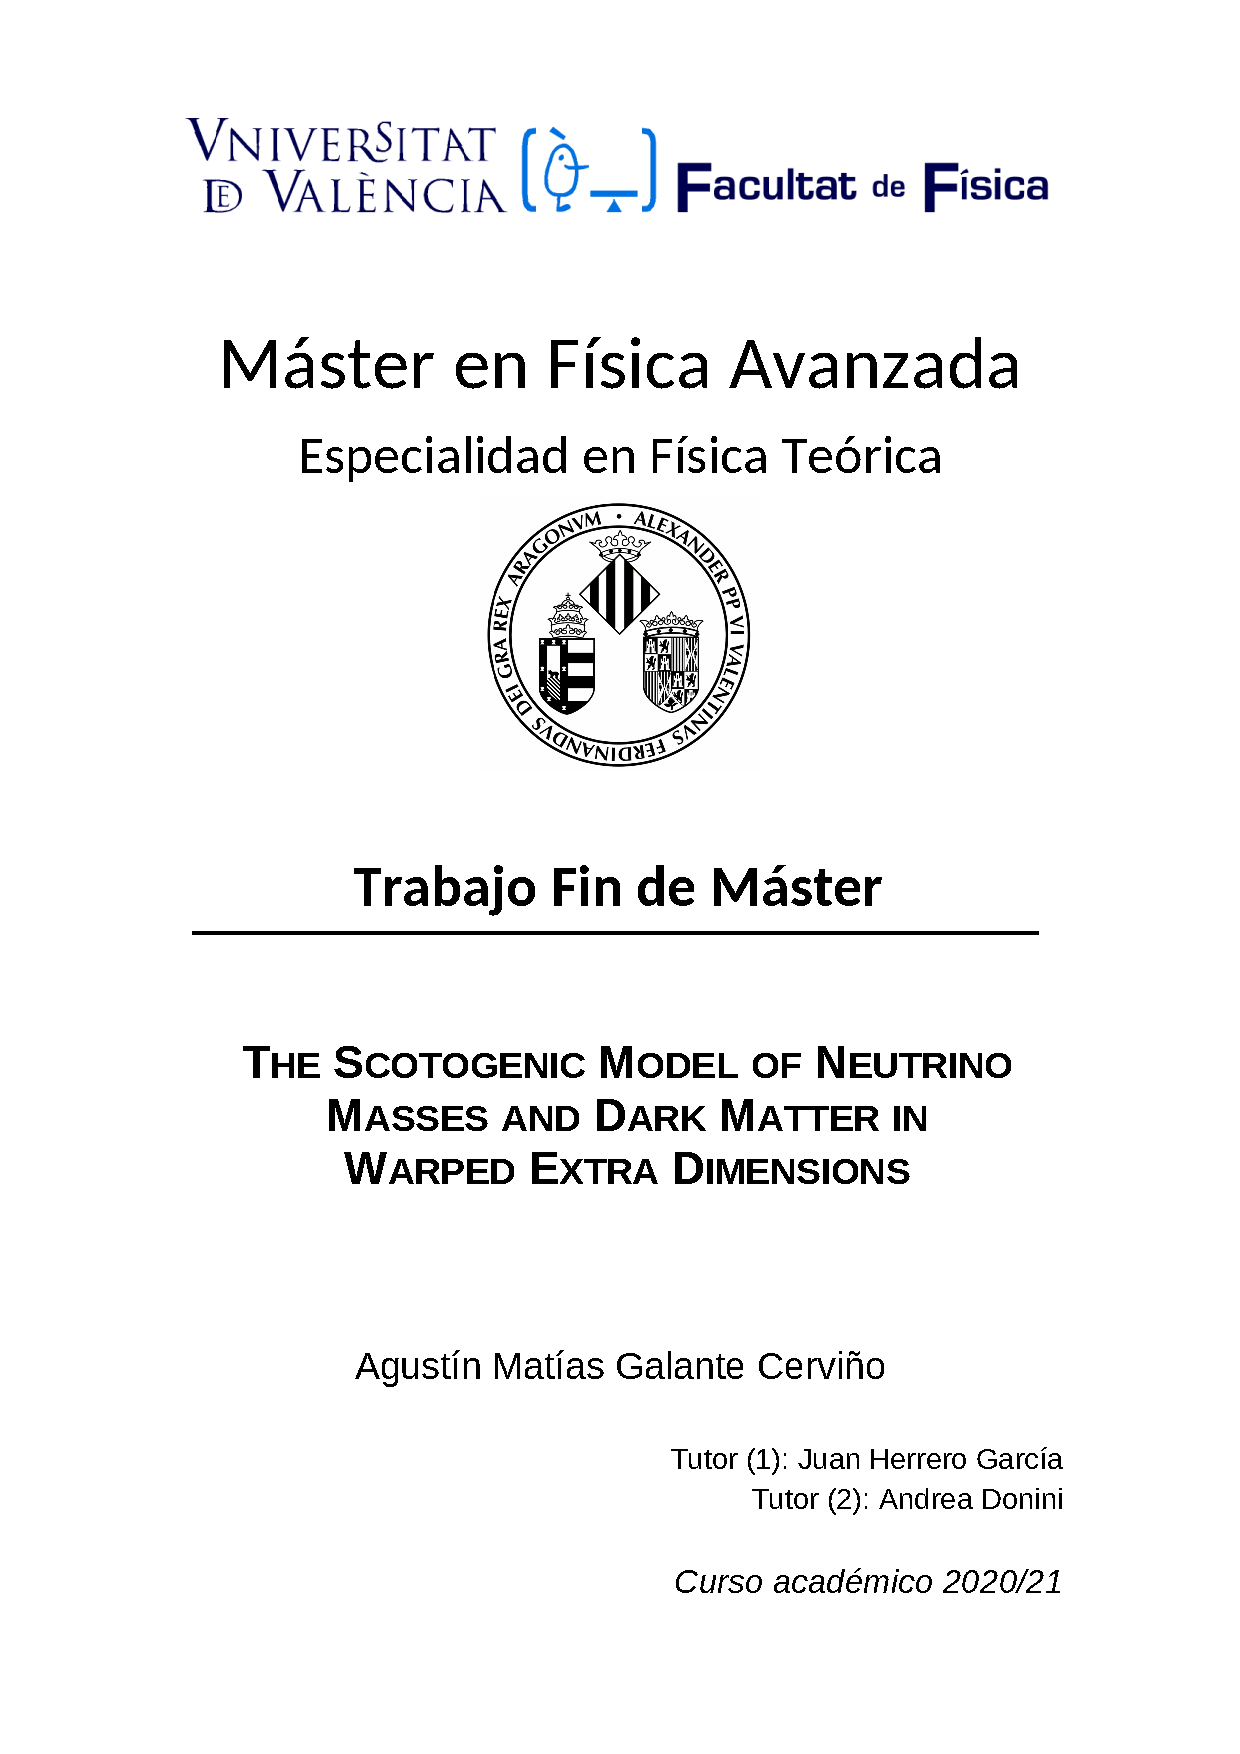
\includepdf{./Portada TFM.pdf}

\section*{Resumen}
En este Trabajo de Fin de Máster se tiene como objeto de estudio la aplicación del modelo
escotogénico, que explica la generación de masas de neutrinos y materia oscura, en el contexto del
escenario Randall-Sundrum, donde se añade una dimensión espacial adicional compactificada al espacio
de Minkowski usual. Comenzaremos revisando brevemente cada uno de estos conocidos modelos según se
encuentran en la literatura, antes de combinarlos y empezar a explorar algunas de las implicaciones
de semejante modelo.

\section*{Abstract}
This Master's Thesis has, as a subject of study, the embedding of the scotogenic model, which
explains the generation of neutrino masses and dark matter, in the context of the Randall-Sundrum
scenario, where an extra compactified spacelike dimension is added to the usual Minkowski space. We
shall start by briefly reviewing both of these known models as seen in the literature, before
combining them and start to explore some of the implications of such an embedding.
\clearpage

\tableofcontents
\clearpage

\chapter{Introduction}
% Aqui motivar que las masas de los neutrinos, materia oscura, y problema de la jerarquía son problemas del MS.
The past three decades have seen an enormous amount of additional vindication to the Standard Model
(SM) of particle physics coming from experimental results, among which is the discovery of the tau
neutrino and the top quark at the TeVatron, and especially the Higgs boson at the LHC, as well as
correctly predicting various properties of previously known particles. Such unquestionable success
is partly shadowed by the many open questions in physics that this model either unsuccesfully
attempted to solve or outright did not consider. Most of these problems are rather pressing, and
have either existed for a long time or have been recently discovered by experiments. Some examples
of these are the observed baryon-antibaryon asymmetry in the Universe, the accelerated expansion of
the latter, and the incompatibility of the SM with a theory of quantum gravity, just to name a few.
The two models we shall consider in this Thesis attempt to solve one or more of these problems.

% - Scotogenic model explica neutrino masses y dark matter.
Neutrinos are considered to be massless in the SM, however two decades ago their oscillation between
flavor eigenstates was confirmed, something that is only possible if at least two out of the three
neutrinos had mass eigenstates not corresponding with their flavor. There are simple ways to
generate these masses, however the smallness of the parameters involved strongly suggests that more
complex mechanisms may be at play. The scotogenic model (ScM) \cite{ma2006verifiable} provides a
possible mechanism for the generation of these masses, extending the scalar sector of the SM as well
as the fermionic one, also introducing a \(Z_2\) symmetry, and generating the neutrino mass matrix at
the one-loop level. This model happens to provide a massive stable particle, weakly
interacting with the rest of the SM, which could also explain the nature of dark matter, a
different, longstanding open question.

% - RS arregla hierarchy problem (explicar como).
% ED sirven para hacer parametros de un modelo naturalmente pequenos.
Models with extra dimensions have been studied for a long time, having seen a major flare in
popularity with the advent of string theory. One such model is the Randall-Sundrum (RS) scenario
\cite{randall1999large}, which includes just one additional, warped compactified dimension along
with constant energy densities at various locations. This allows for a natural solution of the
hierarchy problem; the implementation of this scenario leads to an exponential scaling of
dimensionful parameters of quantum field theories, allowing them to be originally near the Planck
scale \(M_{Pl}\), ending up with values near the expected electroweak scale in our universe while
introducing a very small discrepancy between \(M_{Pl}\) and \(M_5\), the latter being the
fundamental scale of gravity in this model. Its attractiveness lies not only in its simplicity, but
also in the relatively lax tuning required of most parameters it introduces.

% - Combinados ademas ayudan a tener fermionic DM (dejado para el futuro). 
% Se puede hacer lambda5 muy pequeno (para tener masas de neutrinos pequenas) poniendo eta en el bulk?
In this Thesis, we implement an embedding of the scotogenic model in the Randall-Sundrum scenario,
looking to put the new particles the former introduces in extradimensional space, while keeping
every SM field in our observable subspace, our 3-brane. The main motivation for doing this is to
allow for the exploration of the possibility of having fermionic dark matter as given by the ScM in
agreement with the observed relic abundance, which is lower than what most of parameter space allows
\cite{Vicente_2015}, while keeping lepton flavor violating processes' widths comfortably within
experimental bounds. Here, we lay down the necessary machinery needed to do such a thing within the
framework of the lower-dimensional effective field theory, obtained once the fifth dimension is
integrated over in the action. This work is organized as follows: Chapter 2 will introduce the
scotogenic model along with calculating two processes used later and a summary of the problems it
might face; Chapter 3 offers an introduction of the Randall-Sundrum scenario and relevant
consequences of its implementation; In Chapter 4 we will study the dynamics of free fields in five
dimensions as well as their interactions with fields confined to branes; In Chapter 5 we will
explore how the two processes calculated for Chapter 2 are modified, and in Chapter 6 we will
finally conclude this Thesis, outlining future work to be done.
\clearpage

\chapter{The scotogenic model}
\label{chap:scm}
It is perfectly possible to grant mass to neutrinos by extending the SM with Yukawa interaction
terms analogous to those used with quarks and charged leptons, making them interact with new
sterile, right-handed neutrinos. However, theoretically it is desireable not to have extremely small
couplings (\(<10^{-12}\)), which is necessary in this case to fit observations, so it is strongly
believed that such a disparity with other Yukawa couplings indicates that the mechanism involved is
more complex than this extension. As a result, a myriad of models sprung up in the past 40 years
aiming to provide a more compelling way of resolving this problem.

% Here, its virtues with respect to other models should be explained
The scotogenic model \cite{ma2006verifiable} in particular is a rather popular solution to this
issue, which has been extensively studied and extended in literature. Its popularity stems from
several attractive features; it is one of the most minimal radiative mass models, and the fact that
it generates neutrino masses at one-loop and not at tree-level provides a natural way to explain
their smallness, as such processes are more suppressed. The new physics it introduces, additionally,
are TeV-scaled and not GUT-scaled as in standard seesaw models, something which does not introduce
additional hierarchy problems. Not only that, but it also happens to provide a good dark matter
candidate, since there is a lightest stable particle which is very heavy and weakly interacts with
the SM. As a matter of fact, this model is named as such in parts of the literature precisely
because of this; \textit{scotos} (\(\sigma \kappa o \tau o \sigma\)) means \say{darkness},
\textit{genein} (\(\gamma \eta \nu \epsilon \iota \nu\)) means \say{produced by}, so \say{produced
by darkness}.

\vspace{-1.5ex}
\section{Premise and objectives}
The scotogenic model consists in the generation of neutrino masses through the coupling at the
one-loop level of neutrinos with the SM Higgs doublet, \(\Phi\), through various new particles,
these being a scalar doublet under \(SU(2)_L\), \(\eta\), and more than one fermionic singlet,
\(N_s\). In order to accomplish this, an exact \(Z_2\) symmetry is introduced as well. If the
scalar potential, now containing both the SM Higgs and this doublet, is to respect this symmetry,
then the bilinear term mixing both fields, \(\Phi^{\dagger}\eta\), has to be forbidden (this term
would otherwise have been able to give neutrinos mass at tree level). 

Representations of the fields we will use in this Thesis are given in table \ref{tab:rep}.
All fermionic fields listed are understood to be left-handed, save for the fermionic
singlets and the charge conjugated fields of charged leptons, which are right-handed.
\vspace{-2ex}
\begin{table}[H]
\begin{center}
\caption{Representations of \(SU(2)_L \times U(1)_Y \times Z_{2}\) of fields relevant to the scotogenic model.}
\vspace{2ex}
% l are left centered columns, c centered, r right centered
\begin{tabular}{|l|l|}
\hline
Multiplet & Representations \\ \hline
\(L_i\) = \((\nu_i, l_i)^T\) & \((2, -1/2, +)\) \\ \hline
\(l^c_i\) & \((1, -1, +)\) \\ \hline
\(\Phi\) = \((\phi^{+}, \phi^{0})^T\) & \((2, 1/2, +)\) \\ \hline
\(\widetilde{\Phi}\) = \((\phi^{0*}, -\phi^{-})^T\) & \((2, -1/2, +)\) \\ \hline
\(\eta\) = \((\eta^{+}, \eta^{0})^T\) & \((2, 1/2, -)\) \\ \hline
\(\widetilde{\eta}\) = \((\eta^{0*}, -\eta^{-})^T\) & \((2, -1/2, -)\) \\ \hline
\(N_{i}\) & \((1, 0, -)\) \\ \hline
\end{tabular}
\label{tab:rep}
\end{center}
\end{table}
\vspace{-3ex}
Considering these representations and the imposition of gauge invariance of the resulting
Lagrangian, one can see that the Yukawa interactions of this model are
\begin{equation}
\Lagr \supset f_{ij} \overline{L}_i \Phi l^c_j + h_{ij} \overline{L}_i \widetilde{\eta} N_j + \hc =
f_{ij} (\overline{\nu}_i \phi^+ + \overline{l}_i\phi^0) l^c_{j} +
h_{ij} (\overline{\nu}_i \eta^{0*} - \overline{l}_i\eta^-) N_j + \hc ,
\label{eq:yukawas}
\end{equation}
and the most general scalar potential is
\begin{equation}
\begin{aligned}
V(\Phi, \eta) = m^2_1 \Phi^{\dagger}\Phi + m^2_2 \eta^{\dagger}\eta
+ \frac{1}{2}\lambda_1(\Phi^{\dagger}\Phi)^2
+ \frac{1}{2}\lambda_2(\eta^{\dagger}\eta)^2 \\
+ \lambda_3(\Phi^{\dagger}\Phi)(\eta^{\dagger}\eta)
+ \lambda_4(\Phi^{\dagger}\eta)(\eta^{\dagger}\Phi)
+ \frac{1}{2}\lambda_5[(\Phi^{\dagger}\eta)^2 + \hc].
\label{eq:scalars}
\end{aligned}
\end{equation}
The fermionic singlets also admit a Majorana mass term, \(\frac{1}{2}M_s\overline{N^c_s} N_s\), a
necessary component as otherwise the active neutrino mass matrix is not generated. Here,
\(N^c_s \equiv \mi \sigma_2 N^*_s\) is the charge conjugated fermionic singlet field.

The Higgs picks up a non-zero VEV just as it does in the SM, so we have that \(m^2_1 < 0\), however
\(\eta\) does not, so \(m^2_2 > 0\). As a matter of fact, it cannot pick up a non-zero VEV as it
would spontaneously break this \(Z_2\) symmetry. It's worth noting that \(\lambda_5\) can be chosen
real without loss of generality thanks to gauge invariance, by making the appropriate transformation
under \(SU(2)_L\). \(\lambda_3\) and \(\lambda_4\) are always real as the terms are already
Hermitian.

The dark matter candidate we previously mentioned could either be the lightest \(N_s\), the real or
the imaginary part of \(\eta^0\), since \(\eta^0\)'s mass eigenstates are these, as we'll see up
next.

\section{Calculating the neutrino mass matrix}
\label{sec:massmat}
Most neutrino mass generation models intend to be as minimal as possible. A natural consequence of
this is that a portion of these models attempt to couple the SM Higgs to active neutrinos somehow.
Regardless of the specifics of such models, it is reasonable to first consider an effective field
theory only containing known particles, as it is almost always guaranteed that the new ones will
become observable at higher energy scales.

The Weinberg operator is an irrelevant term of the SM Lagrangian when considered as an effective
field theory. It is the lowest dimension operator resulting in the generation of Majorana
mass terms for active neutrinos after electroweak symmetry breaking (EWSB),
\begin{equation}
\frac{h_{ij}}{\Lambda} \overline{L}_{L,i} \widetilde{\Phi} L^c_{L,j} \widetilde{\Phi} + \hc
\rightarrow \frac{h_{ij}}{2 \Lambda} v^2 \: \overline{\nu}_i \nu^c_j + \hc.
\end{equation}
In this case, as active neutrinos are left-handed, their charge conjugated fields are
\(\nu^c_i \equiv -\mi\sigma_2\nu^*_i\). The scotogenic model thus provides the following realization
of this effective operator. The new interaction terms in eq. (\ref{eq:yukawas}) and
(\ref{eq:scalars}) allow for the following process to occur:
\begin{figure}[H]
\centering
\begin{tikzpicture}
\begin{feynman}
\vertex (i) {\(\nu_{i}\)};
\vertex[right=1.6cm of i] (a);
\vertex[right=2.2cm of a] (b);
\vertex[right=1.6cm of b] (f) {\(\nu_{j}\)};
\vertex[right=1.1 of a] (aux);
\vertex[above=1.65cm of aux] (c);
\vertex[above=3.3cm of a] (d) {\(\phi^0\)};
\vertex[above=3.3cm of b] (e) {\(\phi^0\)};

\diagram*{
(i) -- [fermion] (a) -- [majorana, edge label'=\(N_{k}\), /tikzfeynman/momentum/arrow style=small] (b) -- [anti fermion] (f),
(a) -- [scalar, edge label=\(\eta^{0}\)] (c) -- [scalar] (e),
(b) -- [scalar, edge label'=\(\eta^{0}\)] (c) -- [scalar] (d),
};
\end{feynman}
\end{tikzpicture}
\vspace{-2ex}
\caption{Feynman diagram of the process responsible for giving mass to neutrinos.}
\label{fig:scmmass1}
\end{figure}
We are after the correction to the neutrino propagator that this process induces. Before we do that,
let us consider the Lagrangian after EWSB, so we will replace \(\Phi\) for its VEV,
\(\langle \Phi \rangle^T = (0, v/\sqrt{2})\), with \(v \simeq 246\) GeV being the measured VEV of
the surviving, real SM Higgs field. The scalar potential detailed above, disregarding the part
depending only on
\(\Phi\), becomes
\begin{equation}
\begin{aligned}
& V\left(\frac{v}{\sqrt{2}}, \eta\right) \supset m^{2}_{2}(\eta^{+*} \eta^{+} + \eta^{0*} \eta^{0}) + \frac{\lambda_{2}}{2} (\eta^{+*} \eta^{+}
+ \eta^{0*} \eta^{0})^{2} \\
&+ \lambda_{3}\langle \phi^0 \rangle^{2}(\eta^{+*} \eta^{+} + \eta^{0*} \eta^{0}) + \lambda_{4}\langle \phi^0 \rangle^{2}\eta^{0*} \eta^{0}
+ \frac{1}{2}\lambda_{5}\langle \phi^0 \rangle^{2}[(\eta^{0})^{2} + (\eta^{0*})^{2}] \\
&= (m^{2}_{2} + \lambda_{3}\langle \phi^0 \rangle^{2}) \eta^{+*} \eta^{+} + \frac{\lambda_{2}}{2} (\eta^{+*} \eta^{+})^{2} \\
&+ \langle \phi^0 \rangle^{2}(\lambda_{3} + \lambda_{4}) \eta^{0*} \eta^{0} + \frac{\lambda_{5}\langle \phi^0 \rangle^{2}}{2}[(\eta^{0})^{2} + (\eta^{0*})^{2}]
+ \frac{\lambda_{2}}{2} (\eta^{0*} \eta^{0})^{2} \\
&+ \lambda_{2} (\eta^{+*} \eta^{+} \eta^{0*} \eta^{0}),
\end{aligned}
\end{equation}
where we took \(\langle \phi^0 \rangle = v/\sqrt{2}\). Observe that while \(\eta^+\)'s mass terms
are obtained straightfowardly just by looking at the potential, \(\eta^0\) has quadratic couplings
not corresponding to a mass term, and as such this is not the mass eigenstate. It's necessary to
redefine this field in order to use the correct propagators in our one-loop calculation. We make use
of two real fields, which are the real and imaginary part of \(\eta^0\),
\(\eta^0 = \frac{1}{\sqrt{2}}(\eta^0_R + \mi \eta^0_I)\) and
\(\eta^{0*} = \frac{1}{\sqrt{2}}(\eta^0_R - \mi \eta^0_I)\).
The masses we obtain are
\begin{equation}
\begin{aligned}
m^2(\eta^{\pm}) \equiv m^2_{\eta} &= m^2_2 + \lambda_3 \langle \phi^0 \rangle^2\\
m^2(\eta^0_R) \equiv m^2_R &= m^2_2 + (\lambda_3 + \lambda_4 + \lambda_5) \langle \phi^0 \rangle^2\\
m^2(\eta^0_I) \equiv m^2_I &= m^2_2 + (\lambda_3 + \lambda_4 - \lambda_5) \langle \phi^0 \rangle^2,
\end{aligned}
\end{equation}
and the Yukawa interactions using the field redefinitions are the following 
\begin{equation}
\begin{aligned}
\Lagr \supset h_{ij} \overline{\nu}_i \eta^{0*} N_j + \hc = h_{ij} \overline{\nu}_i \eta^0_R N_j
- \mi h_{ij} \overline{\nu}_i\eta^0_I N_j + \hc ,
\label{eq:yukscm}
\end{aligned}
\end{equation}
so we see that not much changes, aside from a relative sign and a factor of i. This factor will
play out a critical role when calculating the mass matrix.

Having settled this matter, we may ignore the coupling to the surviving Higgs field and merely
consider \(\eta^0_R\) and \(\eta^0_I\) with their new masses, so we end up dealing with
\(2n_{fs}\) self-energy diagrams as depicted in figure \ref{fig:scmmass2}, \(n_{fs}\) being the
number of fermionic singlets.
\vspace{-2ex}
\begin{figure}[H]
\centering
\[\mathlarger{\mathlarger{\mathlarger{\sum_{s}}}}
\feynmandiagram [large, baseline=(d.base), layered layout, horizontal=b to c] {
a [particle=\(\nu_i\)] -- [fermion, momentum=\(p\)] b -- [scalar, half left, looseness=1.5, momentum=\(p+k\), edge label'=\(\eta^0_R\)] c
-- [majorana, half left, looseness=1.5, momentum=\(k\), edge label'=\(N_s\)] b,
c -- [anti fermion, momentum=\(p\)] d [particle=\(\nu_j\)],
}; +
\feynmandiagram [large, baseline=(d.base), layered layout, horizontal=b to c] {
a [particle=\(\nu_i\)] -- [fermion, momentum=\(p\)] b -- [scalar, half left, looseness=1.5, momentum=\(p+k\), edge label'=\(\eta^0_I\)] c
-- [majorana, half left, looseness=1.5, momentum=\(k\), edge label'=\(N_s\)] b,
c -- [anti fermion, momentum=\(p\)] d [particle=\(\nu_j\)], 
};
\]
%\feynmandiagram [large, baseline=(d.base), layered layout, horizontal=b to c] {
%a [particle=\(\nu_i\)] -- [fermion, momentum=\(p\)] b -- [scalar, half left, looseness=1.5, momentum=\(p+k\), edge label'=\(\eta^0_R/\eta^0_I\)] c
%-- [majorana, half left, looseness=1.5, momentum=\(k\), edge label'=\(N_s\)] b,
%c -- [anti fermion, momentum=\(p\)] d [particle=\(\nu_j\)],
%};
\caption{Diagram of the resulting self-energy process after EWSB from fig. \ref{fig:scmmass1}.}
\label{fig:scmmass2}
\end{figure}
Details on the calculation of the mass matrix have been laid out in appendix \ref{app:massmat}.
We obtain the following,
\begin{equation}
\begin{aligned}
\begin{gathered}
(m_{\nu})_{ij} = \sum_{s}\frac{h_{is}h_{js} M_s}{16\pi^2}\left( \frac{m^2_R}{m^2_R - M^2_s}\ln \frac{m^2_R}{M^2_s} -
\frac{m^2_I}{m^2_I - M^2_s}\ln \frac{m^2_I}{M^2_s} \right),
\label{eq:massmat}
\end{gathered}
\end{aligned}
\end{equation}
where the mass of the singlet neutrino \(N_s\) is \(M_s\), with \(s = 1, 2, 3\) being a flavor
index. Experimental data can be reproduced correctly with TeV scale masses and a very small mass
splitting between \(\eta^0_R\) and \(\eta^0_I\), given by
\(m^2_R - m^2_I = 2 \lambda_5 \langle \phi^0 \rangle^2\), which in turn implies small \(\lambda_5\).
With this, we can simplify eq. (\ref{eq:massmat}),
\begin{equation}
\begin{aligned}
\begin{gathered}
(m_{\nu})_{ij} = \frac{\lambda_5 \langle \phi^0 \rangle^2}{8 \pi^2}\sum_s \frac{h_{is}h_{js} M_s}{m^2_0 - M^2_s}
\left( 1 - \frac{M^2_s}{m^2_0 - M^2_s}\ln \frac{m^2_0}{M^2_s} \right),
\label{eq:massmatsimp}
\end{gathered}
\end{aligned}
\end{equation}
where \(m^2_0 = (m^2_R + m^2_I)/2\).

\section{Exploring lepton flavor violation}
\label{sec:lfv}
As long as neutrinos have mass eigenstates not corresponding with flavor eigenstates
(so \(U_{\PMNS} \neq I\)) there exists the possibility of lepton flavor violation,
so neutrino mass generation goes hand-in-hand with considering the possibility of processes
like \(\mu \rightarrow e\) in nuclei, or \(\tau \rightarrow \mu \gamma\) to occur.
The process with the most stringent experimental limits is \(\mu \rightarrow e \gamma\), so it's a
good idea to start considering its phenomenology within novel models like the one at hand.

The effective Lagrangian describing this decay is \cite{Beneke_2016}
\begin{equation}
\begin{aligned}
\begin{gathered}
\Lagr_{l_i \rightarrow l_j \gamma} = A_R m_i \overline{l}_j \sigma^{\mu \nu}F_{\mu \nu} P_R l_i
+ A_L m_i \overline{l}_j \sigma^{\mu \nu}F_{\mu \nu} P_L l_i + \hc \\
= A_R m_i \overline{l}_{j,L} \sigma^{\mu \nu}F_{\mu \nu} l_{i,R}
+ A_L m_i \overline{l}_{j,R} \sigma^{\mu \nu}F_{\mu \nu} l_{i,L} + \hc ,
\label{eq:efflagremu}
\end{gathered}
\end{aligned}
\end{equation}
where \(F_{\mu \nu}\) is the electromagnetic field strength tensor and \(P_L\) and \(P_R\) are the
chirality projectors. The subindex \(i\) denotes the heavier lepton, in our case the muon, and \(j\)
the lighter one, here the electron. The couplings of each of these terms are
\begin{equation}
A_R = - \frac{e(F_2 (0) - \mi F_3(0))}{4m^2_{i}}; \quad A_L = - \frac{e(F_2 (0) + \mi F_3(0))}{4m^2_{i}}.
\label{eq:aral}
\end{equation}
\(F_2(p^2)\) and \(F_3(p^2)\) are form factors as defined in the context of the invariant vertex function,
the template for which is
\begin{equation}
\begin{aligned}
\Gamma^{\mu} = - \mi e \overline{u}_{l_j} (q_2, r_2) \Bigg[\gamma^{\mu} F_1(p^2) +
\frac{\mi \sigma^{\mu \nu}p_{\nu}}{2 m_i}F_2(p^2) + \frac{\sigma^{\mu \nu}p_{\nu}}{2 m_i}\gamma_5 F_3(p^2)
+ (p^2 \gamma^{\mu} - \slashed{p} p^{\mu}) \gamma_5 F_4(p^2)\Bigg]u_{l_i} (q_1, r_1).
\label{eq:template}
\end{aligned}
\end{equation}
\vspace{-3ex}
\begin{figure}[H]
\centering
\[\scalebox{0.9}{
\begin{tikzpicture}
\begin{feynman}
\vertex (i) {\(l_i\)};
\vertex[right=1.75cm of i] (loop1);
\vertex[right=2.5cm of loop1] (loop2);
\vertex[right=1.75cm of loop2] (qed);
\vertex[right=2cm of qed] (aux1);
\vertex[above=2cm of aux1] (f1) {\(\gamma\)};
\vertex[below=2cm of aux1] (f2) {\(l_j\)};

\diagram*{
(i) -- [fermion, momentum=\(q_1\)] (loop1) -- [fermion, edge label=\(N_{s}\), rmomentum'=\(k\)] (loop2) -- [fermion, momentum=\(q_1\)] (qed) -- [photon, rmomentum=\(p\)] (f1),
(qed) -- [fermion, momentum=\(q_2\)] (f2),
(loop1) -- [scalar, quarter left, out=90, in=90, looseness=2.0, edge label'=\(\eta^{-}\), momentum=\(q_1+k\)] (loop2),
};
\end{feynman}
\end{tikzpicture}
\begin{tikzpicture}
\begin{feynman}
\vertex (i) {\(l_i\)};
\vertex[right=2.5cm of i] (qed);
\vertex[right=1cm of qed] (aux1);
\vertex[right=3cm of qed] (aux2);
\vertex[right=4.2cm of qed] (aux3);
\vertex[below=0.9cm of aux1] (loop1);
\vertex[below=2.5cm of aux2] (loop2);
\vertex[above=3cm of aux3] (f1) {\(\gamma\)};
\vertex[below=3.2cm of aux3] (f2) {\(l_j\)};

\diagram*{
(i) -- [fermion, momentum=\(q_1\)] (qed) -- [photon, rmomentum=\(p\)] (f1),
(qed) -- [fermion, momentum=\(q_2\)] (loop1) -- [fermion, edge label=\(N_{s}\), rmomentum'=\(k\)] (loop2) -- [fermion, momentum=\(q_2\)] (f2),
(loop1) -- [scalar, quarter left, out=90, in=90, looseness=2.0, edge label'=\(\eta^{-}\), momentum=\(q_2+k\)] (loop2),
};
\end{feynman}
\end{tikzpicture}
}\]
\[\scalebox{0.9}{
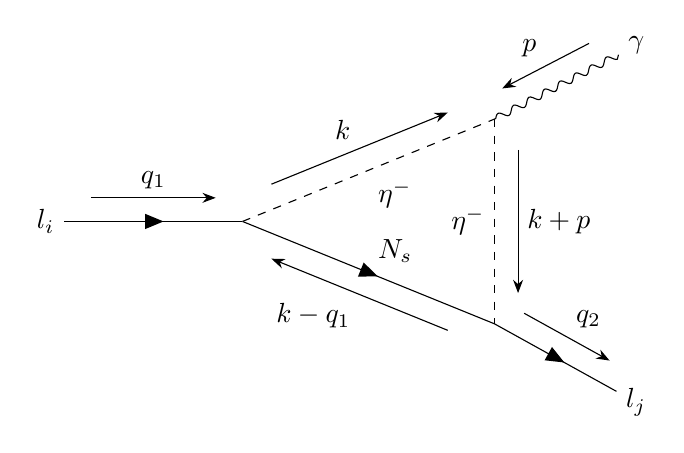
\begin{tikzpicture}
\begin{feynman}
\vertex (i) {\(l_i\)};
\vertex[right=2.5cm of i] (a);
\vertex[right=3.2cm of a] (aux1);
\vertex[above=1.3cm of aux1] (b);
\vertex[below=1.3cm of aux1] (c);
\vertex[right=1.8cm of aux1] (aux2);
\vertex[above=2cm of aux2] (f1) {\(\gamma\)};
\vertex[below=2cm of aux2] (f2) {\(l_j\)};
\diagram*{
(i) -- [fermion, momentum=\(q_1\)] (a) -- [fermion, edge label=\(N_{s}\), rmomentum'=\(k-q_1\)] (c) -- [fermion, momentum=\(q_2\)] (f2),
(a) -- [scalar, edge label'=\(\eta^{-}\), momentum=\(k\)] (b) -- [photon, rmomentum=\(p\)] (f1),
(b) -- [scalar, edge label'=\(\eta^{-}\), momentum=\(k+p\)] (c),
};
\end{feynman}
\end{tikzpicture}
}\]
\vspace{-5ex}
\caption{One-loop diagrams responsible for \(l_i \rightarrow l_j \gamma\).}
\label{fig:egamma}
\end{figure}
The two upper diagrams making this process possible in fig. \ref{fig:egamma} do not contribute to
\(F_2 (p^2)\) nor to \(F_3 (p^2)\), therefore we only have to calculate the lower one's amplitude to
obtain these form factors. The vertex for the uppermost interaction in the diagram we'll use is
\(\mi e [k - (-k - p)]_{\mu} = \mi e (2k + p)_{\mu}\) \cite{Romao_2012}. Details of the calculation
of this process' amplitude have been laid out in appendix \ref{app:lfv}. The resulting expression
for the branching ratio up to powers of the electron mass is \cite{Beneke_2016}
\begin{equation}
\begin{aligned}
\mathrm{BR}(\mu \rightarrow e \gamma) = \frac{m^5_{\mu}}{4\pi\Gamma_{\mu}}(|A_L|^2 + |A_R|^2),
\label{eq:muegammabr}
\end{aligned}
\end{equation}
where \(\Gamma_{\mu} \approx G^2_F m^5_{\mu}/(192\pi^3)\) is the total decay width of the muon. 
\(F_2(p^2=0)\) and \(F_3(p^2=0)\) as outlined in eq. (\ref{eq:template}) are
\begin{equation}
\begin{aligned}
\begin{gathered}
F_2(p^2 = 0) = -\frac{m^2_{\mu}}{8\pi^2 m^2_{\eta}} \sum_s h_{\mu s} h^*_{e s}
\left(\frac{1 - 6x_s + 3x_s^2 + 2x_s^3 - 6x_s^2 \ln x_s}{6(1-x_s)^4}\right) \\
\equiv -\frac{m^2_{\mu}}{8\pi^2 m^2_{\eta}} \sum_s h_{\mu s} h^*_{e s} F(x_s) \\
F_3(p^2) = \mi F_2(p^2),
\label{eq:formfactors}
\end{gathered}
\end{aligned}
\end{equation}
where \(x_s \equiv M^2_s/m^2_{\eta}\). We have that
\begin{equation}
\begin{aligned}
A_R = -\frac{e}{2m^2_{\mu}}F_2(0) \quad A_L = 0,
\label{eq:aral2}
\end{aligned}
\end{equation}
which in turn produces
\begin{equation}
\begin{aligned}
\mathrm{BR}(\mu \rightarrow e \gamma) = \frac{m^5_{\mu}}{4\pi\Gamma_{\mu}}\frac{e^2}{4m^4_{\mu}}|F_2(0)|^2
= \frac{m_{\mu}e^2}{16\pi\Gamma_{\mu}}|F_2(0)|^2.
\label{eq:aral3}
\end{aligned}
\end{equation}
The current experimental bound was set by the MEG experiment,
\(\mathrm{BR}(\mu \rightarrow e \gamma) < 4.2 \cdot 10^{-13}\) at 90\% confidence level
\cite{baldini2016search}. The total decay width of the muon is very small,
\(\Gamma_{\mu} \approx 2.996 \cdot 10^{-19}\) GeV, so the factor multiplying \(|F_2(0)|^2\) will be
quite large.
We know the value of each of these parameters in said factor, so we can establish an
upper bound for \(64\pi^4|F_2(0)|^2\), which is made up entirely of scotogenic model parameters
except for the muon mass, kept there to keep the bound dimensionless,
\begin{equation}
\begin{aligned}
64\pi^4|F_2(0)|^2 < \frac{1024\pi^5\Gamma_{\mu}}{m_{\mu}e^2} \cdot 4.20 \cdot 10^{-13} = 4.07 \cdot 10^{-24}.
\label{eq:bound}
\end{aligned}
\end{equation}

One can gather from eq. (\ref{eq:formfactors}) that the smallness of this branching ratio will arise
from the interplay between \(F(x_s)\) and the factor of \(1/m^2_{\eta}\), if we wish to have
decently sized Yukawa couplings, between 0.1 and 1. It doesn't seem trivial to probe this function's
behaviour at first glance, so a plot ought to help,

\begin{figure}[H]
\centering
\includegraphics[width=\linewidth, width=0.6\textwidth, height=!]{../Figure_2.png}
\caption{Plot of \(\frac{m^2_{\mu}}{m^2_{\eta}}F(x_s)\) as a function of \(m_{\eta}\) and \(M_s\).
The vertical axis is on a base 10 logarithmic scale, \(m_{\eta}\) and \(M_s\) are on linear scales.}
\label{fig:1xFxs}
\end{figure}

Looking at the bound on eq. (\ref{eq:bound}) and comparing it with fig. \ref{fig:1xFxs}, we
immediately gather that having both masses large enough is sufficient for this function to
guarantee a low enough form factor \(F_2 (0)\) with Yukawa couplings of order 1, the latter being
something needed for \(N_1\) to be dark matter. This is not such an interesting situation, however,
as it will make the direct detection of these new particles at accelerators more difficult.

In order to extract more concrete bounds, let us make a few assumptions. We will take \(x_1 \sim 1\),
and assume that \(F(x_2)\) and \(F(x_3)\) contribute much less to the branching ratio. In fig.
\ref{fig:Fxs2} we plot the behaviour of this function to confirm that we are not being misled,

\begin{figure}[H]
\centering
\includegraphics[width=\linewidth, width=0.6\textwidth, height=!]{../Fxs2.png}
\caption{\(F(x_s)\) between \(x_s\) = 0.01 and \(x_s\) = 10.}
\label{fig:Fxs2}
\end{figure}
These assumptions imply \(x_2, x_3 \gtrsim 10\) if the products of Yukawa couplings
\(h_{\mu 2}h^*_{e 2}\) and \(h_{\mu 3}h^*_{e 3}\) are similar or slightly inferior to
\(h_{\mu 1}h^*_{e 1}\). As such, we could just consider the latter in the branching ratio:
\begin{equation}
\begin{aligned}
\mathrm{BR}(\mu \rightarrow e \gamma) = \frac{m_{\mu}e^2}{16\pi\Gamma_{\mu}}\frac{m^4_{\mu}}{64\pi^4m^4_{\eta}}
\Big|\sum_s h_{\mu s} h^*_{e s} F(x_s)\Big|^2
\approx \frac{m^5_{\mu}e^2}{1024\pi^5\Gamma_{\mu}}\frac{1}{m^4_{\eta}} |h_{\mu 1}|^2 |h^*_{e 1}|^2 |F(x_1 = 1)|^2.
\label{eq:aral4}
\end{aligned}
\end{equation}
Knowing that \(F(x_1 = 1) \approx 0.083\), we have that
\begin{equation}
\begin{aligned}
\begin{gathered}
%\mathrm{BR}(\mu \rightarrow e \gamma) = \frac{m_{\mu}e^2}{16\pi\Gamma_{\mu}}\frac{m^4_{\mu}}{64\pi^4m^4_{\eta}}
%\Big|\sum_s h_{\mu s} h^*_{e s} F(x_s)\Big|^2
\frac{|h_{\mu 1}|^2 |h^*_{e 1}|^2}{m^4_{\eta}} < \frac{1024\pi^5\Gamma_{\mu}}{m^5_{\mu}e^2|F(x_1 = 1)|^2}
\cdot 4.20 \cdot 10^{-13} = 4.74 \cdot 10^{-18} \: \mathrm{GeV}^{-4} \\
\frac{|h_{\mu 1}||h^*_{e 1}|}{m^2_{\eta}} < 2.18 \cdot 10^{-9} \: \mathrm{GeV}^{-2}.
\label{eq:aral5}
\end{gathered}
\end{aligned}
\end{equation}
Finally, this bound translates into the possibilities shown in fig. \ref{fig:metaprime},
\begin{figure}[H]
\centering
\includegraphics[width=\linewidth, width=0.6\textwidth, height=!]{../metaprime.png}
\caption{\(\frac{|h_{\mu 1}||h^*_{e 1}|}{m^2_{\eta}}\) as a function of \(m_{\eta}\). The horizontal
red line represents the experimental upper bound in eq. (\ref{eq:aral5}).}
\label{fig:metaprime}
\end{figure}
We see that these Yukawa couplings, if they're similar, need to be on the order of \(\sqrt{10^{-3}}
\sim 0.03\) or lower so that they yield values of \(m_{\eta}\) which could be reached at accelerators.
\clearpage

\section{Possible issues}
\label{sec:possiss}
Exploration of various kinds of processes harboring both lepton number and lepton flavor violation,
as well as studies of the feasibility of the fermionic singlet being dark matter have been carried
out in the context of this model in \cite{Kubo_2006, Aristizabal_Sierra_2009, Suematsu_2009,
Adulpravitchai_2009}, stressing out the link between these two areas. Especially refs.
\cite{Toma_2014, Vicente_2015} exhaustively explored the parameter space along these lines,
comparing viable values to current and future sensitivity of experiments. These later studies have
resulted in bounds for these parameters that are rather restrictive, expecting future experiments to
be able to rule out major portions of the theory's parameter space, even completely excluding
certain scenarios such as \(N_1-N_1\) annihilation in the early universe. Arguably, this could be
considered to be one of the reasons that have led to the flurry of scotogenic model extensions
\cite{beniwal2020scotosinglet, Ahriche_2016, escribano2021ultraviolet}.

If one balances Yukawa couplings and \(\lambda_5\) such that neutrino masses are correctly
generated, the scenario where there is \(N_1-N_1\) annihilation forces \(\lambda_5\) to have a very
small viable interval of reduced values, from \(10^{-4}\) in Ma's original estimation
\cite{ma2006verifiable} to \(10^{-11} - 10^{-10}\) in \cite{Vicente_2015}. If \(\lambda_5\) is
larger, the stringent upper limits on decay rates into various modes with lepton flavor violation
implies low upper bounds of the Yukawa couplings which puts the hypothesis that this singlet is dark
matter at risk of being false; if these couplings are too small, the cross section for annihilation
or coannihilation with \(\eta\) becomes too small, thus relic density is higher, possibly beyond
what experiments suggest, so this singlet would no longer be a good dark matter candidate.
%On the other hand, if \(\lambda_5\) is smaller, Yukawa couplings have to be larger, likely above the
%perturbativity limit, in fact.
\begin{figure}[H]
\centering
\subfigure[\(h_{ij}\overline{\nu}_{i}\eta^{0}_R N_{j} - \mi h_{ij}\overline{\nu}_{i}\eta^{0}_I N_{j} + \hc\)]{
\begin{tikzpicture}
\begin{feynman}
\vertex (i1) {\(N_{i}\)};
\vertex[below=2.2cm of i1] (i2) {\(N_{k}\)};
\vertex[right=2.2cm of i1] (a);
\vertex[right=2.2cm of a] (f1) {\(\nu_{j}\)};
\vertex[below=2.2cm of a] (b);
\vertex[right=2.2cm of b] (f2) {\(\overline{\nu}_{m}\)};

\diagram*{
(i1) -- [plain] (a) -- [fermion] (f1),
(b) -- [scalar, edge label=\(\eta^{0}_R/\eta^{0}_I\)] (a),
(i2) -- [plain] b -- [anti fermion] (f2) [particle=\(N_{k}\)],
};
\end{feynman}
\end{tikzpicture}
}
\subfigure[\(-h_{ij}\overline{l}_{i}\eta^{-}N_j + \hc\)]{
\begin{tikzpicture}
\begin{feynman}
\vertex (i1) {\(N_{i}\)};
\vertex[below=2.2cm of i1] (i2) {\(N_{k}\)};
\vertex[right=2.2cm of i1] (a);
\vertex[right=2.2cm of a] (f1) {\(l^{-}_{j}\)};
\vertex[below=2.2cm of a] (b);
\vertex[right=2.2cm of b] (f2) {\(l^{+}_{m}\)};

\diagram*{
(i1) -- [plain] (a) -- [fermion] (f1),
(b) -- [scalar, edge label=\(\eta^{\pm}\)] (a),
(i2) -- [plain] b -- [anti fermion] (f2),
};
\end{feynman}
\end{tikzpicture}
}
\caption{Fermionic singlet annihilation channels to leptons given by the scotogenic model.}
\label{fig:scmanni}
\end{figure}

\chapter{Warped additional dimension}
The Randall-Sundrum scenario \cite{randall1999large} was proposed in order to solve the hierarchy
problem, consisting in the following: If we are to believe that SM is not the ultimate theory
(and we have many reasons to do so) then it could be understood as an effective low-energy
theory valid up until an energy scale (in our case, the Planck scale \(M_{Pl}\)), dependent on
familiar, light (relative to said scale) fields. However, physics appearing at higher energy scales
have an effect on dimensionful couplings of the low-energy theory. Irrelevant couplings contain
negative powers of the scale, suppressing them, and relevant couplings have positive powers of this
scale. In the SM, the only relevant coupling we have is the mass term of the Higgs pre-EWSB, and it
is very small compared to the energy scale \(M_{Pl} \sim 10^{19}\) GeV. A finely-tuned cancellation
should happen in these unknown, high-energy physics in order to yield the right VEV (\(\sim 246\)
GeV).

The RS model consists in the addition of a compact space-like dimension to the usual (1+3)-dimensional
space-time with concrete boundary conditions, as well as introducing a bulk\footnote{Interdimensional space.}
cosmological constant (\(\Lambda_5\)) and two brane tensions (\(f_{\IR}, f_{\UV}\)) to each end of
the additional dimension. When tuning the three constants appropriately, one arrives at the following
metric,
\begin{equation}
\md s^2 = \me^{-2 \sigma(\varphi)} \eta_{\mu \nu} \md x^{\mu} \md x^{\nu} - r^2_c\md \varphi^2,
\label{eq:rsmetric}
\end{equation}
where we chose the signature \((+,-,-,-,-)\). The ``warp'' factor, \(\me^{-2 \sigma(\varphi)}\), with
\(\sigma(\varphi) \equiv kr_c |\varphi|\), is what will generate the hierarchy, as we will see up next.
\vspace{-2ex}
\section{The set-up}
Living in a lower-dimensional subspace means that we need to impose boundary conditions on
spacetime, which in this scenario are taken to be periodicity in the fifth dimensional coordinate,
identifying \((x, \varphi)\) with \((x, \varphi + 2\pi)\), and reflectivity, so \((x, \varphi)\) is
identified with \((x, -\varphi)\). This means that the fifth dimension is symmetric under
\(S^1/Z_2\), having the structure of an orbifold and granting it a length of \(\pi r_c\).  \(r_c\)
is a constant with dimensions of length, corresponding to a \textit{compactification radius} before
orbifolding\footnote{Applying the aforementioned boundary conditions.}, and \(\varphi\) is an
adimensional coordinate, akin to an angle. Having established this, we now know that \(k\), the
curvature of space-time along the fifth dimension, has units of energy. We take values of
\(\varphi\) from \(-\pi\) to \(\pi\), even though the metric is entirely defined within
the range \(0 \leq \varphi \leq \pi\). The orbifold fixed points at \(\varphi = 0\) and \(\varphi =
\pi\) will now be the locations of two 3-branes, the UV-\footnote{Also called the hidden or Planck
brane in literature.} and IR-brane\footnote{Also called the visible or TeV brane.}, respectively.
They extend in the directions of the other four dimensions, forming the boundaries of this
five-dimensional space-time, which is a slice of anti-de Sitter space (AdS\({}_5\)). The action
describing this situation is given by
\begin{equation}
\begin{aligned}
S &= S_{\bulk} + S_{\IR} + S_{\UV} \\
S_{\bulk} &= \int \md^4 x \int^{\pi}_{-\pi} \md \varphi \sqrt{G}(-\Lambda_5 - 2M^3_5R) \\
S_{\IR} &= \int \md^4 x \sqrt{-g_{\IR}}(\Lagr_{\mathrm{SM}} - f^4_{\IR}) \\
S_{\UV} &= \int \md^4 x \sqrt{-g_{\UV}}(-f^4_{\UV} + \cdots),
\label{eq:bulkac}
\end{aligned}
\end{equation}
where \(M_5\) is the fundamental scale of gravity, \(G = r^2_c \me^{-8\sigma}\) is the determinant
of the bulk metric \(G_{MN}\) (where \(M,N = 0, \dots, 4\)), \(R\) is the bulk Ricci scalar and
\(g_{\IR}\), \(g_{\UV}\) are the determinants of the 4-dimensional components of the bulk metric
evaluated at each of the branes,
\begin{equation}
\begin{aligned}
g^{\IR}_{\mu \nu} (x) \equiv G_{\mu \nu}(x, \varphi = \pi)
\quad g^{\UV}_{\mu \nu} (x) \equiv G_{\mu \nu}(x, \varphi = 0).
\end{aligned}
\end{equation}
The observable universe, which we live in, is then confined to the IR-brane, while we merely assume
that, aside from the tension, the UV-brane contains physics suppressed by the Planck scale,
which is too high for us to observe, thus we will not consider them.

If the metric in eq. (\ref{eq:rsmetric}) is to be a solution of the Einstein field equations, then
the brane tensions must be equal to
\begin{equation}
f^4_{\IR} = -f^4_{\UV} = \sqrt{-24 M^3_5 \Lambda_5},
\end{equation}
in order to cancel \(\Lambda_5\). It is worth noting that imposing this metric as a solution also
implies that \(k < M_5\).

\section{Kaluza-Klein expansion of the graviton}
For reasons we will discuss shortly, it becomes necessary to consider an effective field theory
of the gravitational fluctuations around the Minkowski metric. We first need to expand the 4-dimensional
components of the metric tensor, and at first order we get
\begin{equation}
G_{\mu \nu}(x, \varphi) = \me^{-2\sigma}\left(\eta_{\mu \nu} + \frac{2}{M^{3/2}_5}h_{\mu \nu}(x, \varphi)\right),
\label{eq:perme}
\end{equation}
where \(h_{\mu \nu}\) is our graviton field, representing the gravitational fluctuations with respect to flat
space-time. We can decompose this field into its modes, forming a Kaluza-Klein (KK) tower \cite{Kaluza_2017, Oskar_2013},
\begin{equation}
h_{\mu \nu}(x, \varphi) = \frac{1}{\sqrt{r_c}}\sum^{\infty}_{n=0} h^{(n)}_{\mu \nu}(x) \chi^{(n)}(\varphi),
\end{equation}
where \(h^{(n)}_{\mu \nu}(x)\) are the KK-modes of the graviton and \(\chi^{(n)}(\varphi)\)
the corresponding wavefunctions. Obtaining a relation between the Planck scale \(M_{Pl}\) and the
fundamental scale of gravity \(M_5\) is one of these reasons, and can be done as follows; we only
use the zero-mode in the perturbed metric in eq. (\ref{eq:perme}), which we now plug into \(S_{\mathrm{bulk}}\)
in eq. (\ref{eq:bulkac}), and consider the curvature term
\begin{equation}
16\pi \int \md^4 x \int^{\pi}_{-\pi} \md \varphi \: M^3_5 r_c \me^{-2kr_c |\varphi|} \sqrt{-\overline{g}} \overline{R}
\equiv M^2_{Pl},
\end{equation}
where \(\overline{g}\) and \(\overline{R}\) are the four-dimensional metric tensor determinant and four-dimensional
Ricci scalar as given by the aforementioned zero-mode. Since low-energy fluctuations don't change
the \(\varphi\) dependence, one can integrate over this coordinate, and get
\begin{equation}
\bar{M}^2_{Pl} = M^3_5 r_c \int^{\pi}_{-\pi} \md \varphi \: \me^{-2kr_c|\varphi|} = \frac{M^3_5}{k}(1 - \me^{-2kr_c\pi}),
\label{eq:M5}
\end{equation}
where \(\bar{M}_{Pl} \equiv M_{Pl}/\sqrt{8\pi}\) is the reduced Planck scale. 
From this relation we can see that, if \(k r_c \gg 1\), the dimensionful quantities of the model are
all of the same order, \(M_{Pl} \sim M_5 \sim k\) (differently from other extra-dimensional models
\cite{Arkani_Hamed_1998, Cox_2012}, in which \(M_5 \ll M_{Pl}\)).

We will now explore the coupling of the graviton to matter fields. First, we turn our attention to
the equations of motion for the KK-modes. By using the Einstein field equations, and
considering the transverse-traceless gauge, these \cite{Davoudiasl_2000} are
\begin{equation}
(\eta^{\rho \epsilon}\partial_{\rho}\partial_{\epsilon} + m^2_n)h^{(n)}_{\mu \nu} = 0,
\end{equation}
where \(m_n \geq 0\) are their masses. Using this and the Einstein field equations again, we arrive
at the equation of motion for the wavefunctions,
\begin{equation}
-\frac{1}{r^2_c}\partial_{\varphi} \left(\me^{-4\sigma}\partial_{\varphi}\chi^{(n)}\right) = m^{2}_{n}\me^{-2\sigma} \chi^{(n)}.
\label{eq:wavegrav}
\end{equation}
After manipulating this equation by making the change of variable \(z_n = m_n \me^{\sigma}/k\)
and \(f^{(n)} = \me^{-2\sigma}\chi^{(n)}\) one can see that the equation of motion is
\begin{equation}
\begin{aligned}
z^2_n(\partial^2_{z_n} f^{(n)}) + z_n (\partial_{z_n} f^{(n)})
+ (z^2_n - 4)f^{(n)} = 0,
\label{eq:bessel}
\end{aligned}
\end{equation}
a second-order Bessel equation, the most general solution of which being the following
linear combination
\begin{equation}
\chi^{(n)}(\varphi) = \frac{\me^{2\sigma}}{N_{n}}[J_{2}(z_{n}) + b_{n2} Y_{2}(z_{n})],
\end{equation}
of Bessel functions of the same order. Here, \(N_{n}\) are normalization constants and \(b_{n2}\)
are coefficients to be determined utilizing boundary conditions. If we consider the limits \(m_n/k
\ll 1\), \(\me^{kr_c\pi} \gg 1\) as well as noticing that since eq. (\ref{eq:wavegrav}) is
self-adjoint \(\partial_{\varphi}\chi^{(n)}\) must be continuous at the orbifold fixed points
\cite{Goldberger_1999_bulk}, we can approximate \(b_{n2}\),
\begin{equation}
b_{n2} \approx x^2_{n2} \me^{-2kr_c\pi},
\end{equation}
with \(x_{n2}\) being the \(n\)-th root of the first order Bessel function of the first kind \(J_1\).
Masses of the KK-modes of the graviton depend on such roots, therefore they are not evenly spaced,
\begin{equation}
m_n = k x_{n2}\me^{-kr_c\pi},
\label{eq:roots}
\end{equation}
(however one can show that, for large \(n\), the roots do become equally spaced).
We can figure out the normalization constants by imposing the following orthonormality condition
on the wavefunctions,
\begin{equation}
\int^{\pi}_{-\pi} \md \varphi \: \me^{-2 \sigma} \chi^{(m)}\chi^{(n)} = \delta_{mn},
\end{equation}
and using the same limit as before, we obtain the following,
\begin{equation}
\begin{aligned}
N_0 &\approx - \frac{1}{\sqrt{kr_c}} \\
N_n &\approx   \frac{1}{\sqrt{2kr_c}}\me^{kr_c\pi} J_2 (x_{n2}) \quad \mathrm{for \: n > 0.}
\end{aligned}
\end{equation}

We're now well positioned to properly figure out the coupling of the graviton; since it's a spin-2
field, it can only couple to the energy-momentum tensor, which implies that this term is
non-renormalizable in four dimensions, as its mass dimension is over four. Its coupling constant
depends on the inverse of the fundamental scale of gravity, \(M_5\), as is typical of effective
field theories. We wish to evaluate this interaction at the IR-brane, so first we expand it,
\begin{equation}
\Lagr_{\eff} = - \frac{1}{M^{3/2}_5} T^{\mu \nu} h_{\mu \nu}(x, \varphi = \pi) =
- \frac{1}{M^{3/2}_5 \sqrt{r_c}}T^{\mu \nu} \sum^{\infty}_{n=0} h^{(n)}_{\mu \nu}(x) \chi^{(n)}(\varphi = \pi),
\label{eq:effgrav}
\end{equation}
then we evaluate the wavefunctions at this point in \(\varphi\),
\begin{equation}
\begin{aligned}
\chi^{(0)}(\varphi = \pi) &= \sqrt{kr_c}(1 - \me^{-2kr_c\pi}) = \sqrt{r_c} \frac{M^{3/2}_5}{\bar{M}_{Pl}} \\
\chi^{(n)}(\varphi = \pi) &= \sqrt{kr_c} \me^{kr_c\pi} = \sqrt{r_c} \: \me^{kr_c\pi} \frac{M^{3/2}_5}{\bar{M}_{Pl}},
\end{aligned}
\end{equation}
where we took the limit \(\me^{-2kr_c\pi} \ll 1\), a reasonable approximation. We also used eq.
(\ref{eq:M5}) to insert \(M_{Pl}\). Plugging this last result in eq. (\ref{eq:effgrav}) yields
\begin{equation}
\Lagr_{\eff} = -\frac{1}{\bar{M}_{Pl}}T^{\mu \nu} h^{(0)}_{\mu \nu}
- \frac{1}{\bar{M}_{Pl}\me^{-kr_c\pi}}T^{\mu \nu}
\sum^{\infty}_{n=1} h^{(n)}_{\mu \nu}.
\label{eq:gravint}
\end{equation}
From eq. (\ref{eq:gravint}) we can see how the hierarchy problem is solved in the RS model: even
though SM fields couple with the graviton zero-mode with the usual \(1/M_{Pl}\) suppression, that
makes gravity so feeble with respect to other forces, they actually couple to higher graviton
KK-modes with \(1/\Lambda\), where \(\Lambda \equiv \bar{M}_{Pl}\me^{-kr_c\pi}\). If
\(k r_c \sim 10\), the scale \(\Lambda\) can be as low as the TeV, thus solving the hierarchy
problem.

%We now see why we have taken the trouble; while the zero-mode couples to the energy-momentum
%tensor with the expected strength, higher, massive KK-modes couple to it with far less suppression,
%thanks to the factor \(\me^{-kr_c\pi}\) inducing a scale \(\Lambda \equiv \bar{M}_{Pl}\me^{-kr_c\pi}\). We
%can easily tune this coupling so that it lays closer to the electroweak scale with moderate values of
%\(kr_c\) like the one mentioned earlier, thus these modes may play a role in the phenomenology at
%lower energies.

Since five-dimensional translational invariance is necessarily broken due to the presence of the
branes, the graviphoton (\(h_{\mu 5}\)) and the graviscalar's (\(h_{55}\)) KK-towers are both
absorbed by the graviton's tower in the unitary gauge to get massive spin-2 KK-modes. The zero-mode
of the graviphoton does not participate in this model's phenomenology \cite{randall1999large}. The
graviscalar's zero-mode will however be relevant in the stabilization of the fifth dimension,
something to be discussed in the following.

In models with additional compactified dimensions, one comes across a worrying problem:
having such dimensions induces a Casimir effect acting on the boundaries of the extra-dimensions,
i.e. the place where the branes are located
\cite{Appelquist1983quantumdyn, Appelquist1983quantumeff, dewit1989, Pont_n_2001}.
In particular, a minimal RS scenario would imply that the two branes are attracted one to each
other, thus the size of the extra-dimension shrinks to a point. In order to solve this conundrum
the Goldberger-Wise mechanism was proposed \cite{Goldberger_1999_modulus}, consisting in the
following; if a scalar bulk field \(S\) is added, along with a potential \(V_{S}(S)\), as well as
interaction terms localized to both branes, \(\delta(\varphi = 0)V_{\UV}(S)\) and
\(\delta(\varphi = \pi)V_{\IR}(S)\), we are able to generate an effective potential \(V(\rho)\) for
the four-dimensional field,
\begin{equation}
\rho = f \me^{-\pi k T},
\label{eq:effpot}
\end{equation}
where \(f = \sqrt{-24 M^3_5/k}\) and \(\langle T \rangle = r_c\). The local minima of this
potential are able to yield the desired value of \(kr_c\) without having to fine-tune much.

\(S\) will also have a KK-tower, however we ignore it because it is expected to be heavy
\cite{Goldberger_2000}. The lightest field is a combination of the zero-modes of the graviscalar
and \(S\), which is \(r\), dubbed the radion. It's possible to calculate its mass using the
effective potential in eq. (\ref{eq:effpot}),
\begin{equation}
m^2_r = \frac{k^2 v^2_v}{3 M^3_5} \left(\frac{m^2}{4 k^2} \right)^2 \me^{-2kr_c \pi},
\label{eq:massrad}
\end{equation}
where \(v_v\) is \(S\) evaluated at the IR-brane and the corresponding mass parameter from the
bulk potential \(V(S)\) is \(m\). We have that \(m^2/4k^2 \ll 1\), so the mass of the radion is
far smaller compared to the mass of the KK-graviton's first mode.

Dark matter and SM fields alike interact with the radion, coupling to it through the trace of the
energy-momentum tensor. Even though massless gauge bosons don't contribute to the latter, the radion
couples indirectly to them through quarks, W boson loops, and the trace anomaly.
\clearpage

\section{Dark matter in the RS scenario}
\label{sec:dmrs}
A possible solution to the problems we outlined back in section \ref{sec:possiss} regarding having
the fermionic singlet as a dark matter candidate can be obtained by introducing the RS scenario
alone, without actually putting any new field in the bulk, or any other field for that matter.
Indeed, it was recently shown that the correct relic abundance using a freeze-out mechanism can be
reached in the context of the RS scenario if both the dark matter candidate and SM fields are
confined to the IR-brane. This DM candidate would be a WIMP-like scalar, fermion or a vector field,
with a mass between 4 and 10.5 TeV in the case of the fermion, only interacting gravitationally,
through both massive KK-gravitons as well as the radion \cite{Folgado_2020, Folgado_2021}, something
which in RS might happen much closer to the electroweak scale, as we have seen previously. Such
enhancement of the annihilation rate in the early universe can be attained without any involvement
of parameters like Yukawa couplings or \(\lambda_i\) in the scotogenic model, however it will still
affect bounds on the value of the mass of the fermionic singlet. These works have shown that moderate
values of \(\Lambda\), between 1 and 100 TeV, have been sufficient to generate such a relic abundance.
However, higher values only smooth the hierarchy problem, requiring further model-building to
explain the little hierarchy problem that remains.

There is a caveat regarding some of these results, as it was shown in
\cite{de_Giorgi_2021, degiorgi2021dark} that a diagram contributing to the annihilation of DM into
KK-gravitons (and radions), was not considered in \cite{Folgado_2020, Folgado_2021}, which modifies
the results of the latter works for scalar DM particles. A thorough phenomenological analysis of the
modified results is still underway. This does not apply to fermionic DM; the embedding we're
presently considering needs little modification to utilize a brane-confined \(N_s\) instead of a
bulk one, as we'll see next, since our choice of bulk fermion will yield a field similar to a
brane-confined one. Concievably, such a scenario (with \(\eta\) in the bulk) could be probed as well
with some of the results obtained here.

\chapter{The scotogenic model in Randall-Sundrum}
Following up with what was discussed in section \ref{sec:dmrs}, it is now clear to see that the main
motivation behind embedding the scotogenic model in Randall-Sundrum is to increase the annihilation
rate of the fermionic singlet in the early universe, by opening up new decay channels through
gravitational interaction.

In this chapter, we will explore the implications of considering the new particles introduced by the
scotogenic model as living in the bulk, these being the scalar doublet \(\eta\) and the fermionic
singlets \(N_i\). We first explore the dynamics of free bulk fields in sec.
\ref{sec:newbulk}, the results of which will be used when working with interactions between
these fields and others confined to the IR-brane. This is, in particular, the case of the
interactions between the Higgs field \(\Phi\) and \(\eta\), as well as the Yukawa interactions. Both
will be discussed in sec. \ref{sec:interextra}.

\section{Pushing the new particles into the bulk}
\label{sec:newbulk}

The fact that we have not observed copies of existing SM particles with different mass suggests that
the SM is confined to the IR-brane. The particles introduced in the scotogenic model could
however be very heavy, as they have not been observed so far, thus they may live in the bulk and have
a massive zero-mode (implying a non-zero bulk mass in the case of bosons). Therefore, we need to
properly describe their fields in a higher-dimensional context, as we did in the case of the graviton.

\subsection{Scalar case}
\label{subsec:scalar}
We shall describe in more detail how we got to the graviton's case by starting with the action of a
bulk complex scalar \cite{Goldberger_1999_bulk}, as the process is independent of spin in bosonic fields 
\begin{equation}
\begin{aligned}
S &= \int \md^4 x \int^{\pi}_{-\pi} \md \varphi \sqrt{G} \: \Lagr \\
&= \int \md^4 x \int^{\pi}_{-\pi} r_c \md \varphi \: \me^{-4\sigma}
\left(g^{MN}\partial_{M}\phi^{\dagger}\partial_{N}\phi - m^{2} \phi^{\dagger} \phi \right).
\label{eq:scalaction}
\end{aligned}
\end{equation}
The Lagrangian, when expanded, is then
\begin{equation}
\begin{aligned}
\Lagr &= \me^{2\sigma}\eta^{\mu \nu}\partial_{\mu}\phi^{\dagger}\partial_{\nu}\phi
- \frac{1}{r^2_c}\partial_{\varphi}\phi^{\dagger}\partial_{\varphi}\phi - m^{2} \phi^{\dagger} \phi.
\end{aligned}
\end{equation}
Euler-Lagrange yields
\begin{equation}
\begin{aligned}
\frac{\partial \Lagr}{\partial\phi^{\dagger}} = -m^{2} \phi,
\end{aligned}
\end{equation}
\begin{equation}
\begin{aligned}
&\frac{1}{\sqrt{G}} \partial_M
\left(\sqrt{G}\frac{\partial\Lagr}{\partial(\partial_M
\phi^{\dagger})}\right)
= \me^{4\sigma}G^{\mu \nu}\partial_{\nu}(\me^{-4\sigma}\partial_{\mu}\phi)
- \frac{1}{r^2_c}\me^{4\sigma} \partial_{\varphi}(\me^{-4\sigma}\partial_{\varphi}\phi).
\end{aligned}
\end{equation}
So equating these two last expressions results in
\begin{equation}
\begin{aligned}
G^{\mu \nu} \partial_{\mu}\partial_{\nu}\phi
- \frac{1}{r^2_c}\me^{4\sigma} \partial_{\varphi}\left(\me^{-4\sigma}\partial_{\varphi}\phi\right) + m^{2}\phi
&= 0\\
\rightarrow \eta^{\mu \nu} \partial_{\mu}\partial_{\nu}\phi
- \frac{1}{r^2_c}\me^{2\sigma} \partial_{\varphi}\left(\me^{-4\sigma}\partial_{\varphi}\phi\right) + \me^{-2\sigma}m^{2}\phi
&= 0,
\label{eq:phieq}
\end{aligned}
\end{equation}
now we decompose the field into its Kaluza-Klein modes,
\begin{equation}
\phi(x, \varphi) = \frac{1}{\sqrt{r_c}}\sum^{\infty}_{n = 0} \phi^{(n)}(x) \xi^{(n)}(\varphi),
\label{eq:scalmodes}
\end{equation}
and plugging a mode into eq. (\ref{eq:phieq}) gets us the following after standard manipulations,
\begin{equation}
\begin{aligned}
(\eta^{\mu \nu} \partial_{\mu}\partial_{\nu} + m^{2}_{n}) \phi^{(n)} = 0 \quad
\text{(4D K-G equation)} \\
- \frac{1}{r^2_c}\partial_{\varphi}\left(\me^{-4\sigma}\partial_{\varphi} \xi^{(n)} \right) +
\me^{-4\sigma}m^2\xi^{(n)} = \me^{-2\sigma} m^2_n\xi^{(n)}.
\label{eq:moveqsca}
\end{aligned}
\end{equation}
In other words; if we take the action in eq. (\ref{eq:scalaction}), plug in its mode
decomposition as shown in eq. (\ref{eq:scalmodes}) and impose orthonormality
conditions on the fifth dimensional wavefunctions,\footnote{The fact that eq.
(\ref{eq:moveqsca}) is real means that we can choose its solutions as real too,
without loss of generality.}
\begin{equation}
\begin{aligned}
\begin{gathered}
\int^{\pi}_{-\pi} \md \varphi \: \me^{-2\sigma} \xi^{(n)} (\varphi) \xi^{(m)} (\varphi) = \delta_{nm},
\label{eq:orthoscalar}
\end{gathered}
\end{aligned}
\end{equation}
we get
\begin{equation}
\begin{aligned}
\begin{gathered}
\int \md^4 x \sum^{\infty}_{n=0} [\eta^{\mu \nu} \partial_{\mu} \phi^{(n)}{}^{\dagger} \partial_{\nu} \phi^{(n)}
- m^2_n\phi^{(n)}{}^{\dagger}\phi^{(n)}].
\end{gathered}
\end{aligned}
\end{equation}
So we see that the action reduces to the infinite sum of familiar four-dimensional fields, each
corresponding to a KK-mode with mass \(m_n\), leading to an effective field theory where we can
safely consider our four dimensions alone (albeit the full 5-dimensional theory is recovered when
the complete KK-tower is considered). This result is general for any particle, independent of its
spin. When changing variables to \(z_{n} = m_{n} \me^{\sigma}/k\) and \(f^{(n)} = \me^{-2\sigma}\xi^{(n)}\)
in eq. (\ref{eq:moveqsca}) one obtains almost the same expression as in eq. (\ref{eq:bessel}),
except for the order of the equation, which is now \(2 \rightarrow \nu_{\phi} = \sqrt{4 + m^2/k^2}\).
Thus the solution's normalization constant and coefficients differ as well.

Such coefficients can also be obtained by using a limiting procedure when integrating around
\(\varphi = 0\) (which also leads to the same condition mentioned previously, which is the continuity
of the first derivative of the wavefunctions at the orbifold fixed points),

\begin{equation}
\begin{aligned}
b_{n\nu_{\phi}} = -\frac{2J_{\nu_{\phi}}\left(\frac{m_n}{k}\right)
+ \frac{m_n}{k}J'_{\nu_{\phi}}\left(\frac{m_n}{k}\right)}{2Y_{\nu_{\phi}}\left(\frac{m_n}{k}\right) + \frac{m_n}{k}Y'_{\nu_{\phi}}\left(\frac{m_n}{k}\right)},
\label{eq:bnv}
\end{aligned}
\end{equation}
and the same can be done in order to obtain \(m_n\) when integrating around \(\varphi = \pi\),
\begin{equation}
\begin{aligned}
[2J_{\nu_{\phi}}(x_{n\nu_{\phi}}) + x_{n\nu_{\phi}}J'_{\nu_{\phi}}(x_{n\nu_{\phi}})][2Y_{\nu_{\phi}}(x_{n\nu_{\phi}}\me^{-k r_c \pi})
+ x_{n\nu_{\phi}}\me^{-k r_c\pi}Y'_{\nu_{\phi}}(x_{n\nu_{\phi}}\me^{-k r_c\pi})] \\
- [2Y_{\nu_{\phi}}(x_{n\nu_{\phi}}) + x_{n\nu_{\phi}}Y'_{\nu_{\phi}}(x_{n\nu_{\phi}})][2J_{\nu_{\phi}}(x_{n\nu_{\phi}}\me^{-k r_c \pi})
+ x_{n\nu_{\phi}}\me^{-k r_c\pi}J'_{\nu_{\phi}}(x_{n\nu_{\phi}}\me^{-k r_c\pi})]
= 0,
\label{eq:relation1scalar}
\end{aligned}
\end{equation}
where \(x_{n\nu_{\phi}}\) is the \(n\)-th root of eq. (\ref{eq:relation1scalar}), instead of
\(J_1 (x)\) as in eq. (\ref{eq:roots}). Now, if we take the limit \(\me^{kr_c\pi} \gg 1\), the
previous relation simplifies to
\begin{equation}
\begin{aligned}
2J_{\nu_{\phi}}(x_{n\nu_{\phi}}) + x_{n\nu_{\phi}}J'_{\nu_{\phi}}(x_{n\nu_{\phi}}) = 0.
\label{eq:relsimpsc}
\end{aligned}
\end{equation}
So, if we wish to find the mass spectrum of these 4D KK-modes, we need to numerically solve
eq. (\ref{eq:relsimpsc}) to obtain \(x_{n\nu_{\phi}}\). This last equation however has a root at 0
that the exact expression, eq. (\ref{eq:relation1scalar}), does not have, so one needs to be
careful here. Moreover, by using the orthonormality relation in eq. (\ref{eq:orthoscalar}), we see
that \(N_n\) is
\begin{equation}
\begin{aligned}
N_n = \pm \sqrt{\int^{\pi}_{-\pi} \md \varphi \: \me^{2\sigma} \: \Bigg[J_{\nu_{\phi}}\left(\frac{m_n}{k}\me^{\sigma}\right)
+ b_{n\nu_{\phi}} Y_{\nu_{\phi}}\left(\frac{m_n}{k}\me^{\sigma}\right)\Bigg]^2}.
\end{aligned}
\end{equation}
To finish, it is important to note that \(f^{(n)}\) can be either even or odd under a
\(Z_2\)-transformation in the orbifold, and we need to choose an option. There is a problem with the
odd choice, however \cite{Flachi_2001}; the requirement that the wavefunction be continuous at the
orbifold fixed points means that it would be 0 at these points. In this Thesis we will only be
dealing with bulk fields interacting with fields confined at the IR-brane, meaning that those
interaction terms will contain these wavefunctions evaluated at a fixed point. If they're 0, there
is no interaction at all, a trivial and uninteresting case given our considerations. We will
consider the wavefunctions belonging to the \(\eta\) doublet even from here on out.
\clearpage

\subsection{Fermionic case}
\label{subsec:fermioniccase}
We now turn to the fermionic singlet. The considerations involved in its inclusion in the bulk are
not as clear cut as with the scalars, as various avenues are possible. The original scotogenic model
stipulates that we are obtaining Majorana mass terms for the active neutrinos, so we need the
fermion running in the loop in fig. \ref{fig:scmmass1} to be a Majorana particle.  

There are various ways to go about this when considering bulk fields, however. We ought to consider
the two following options:
\begin{itemize}
\item {\bf Bulk Dirac fermion} \\
The following transformation under orbifold \(Z_2\) of a fermionic bulk field
\begin{equation}
\begin{aligned}
\begin{gathered}
\Psi (x, -\varphi) = \pm \gamma_5 \Psi (x, \varphi),
\label{eq:fermpar1}
\end{gathered}
\end{aligned}
\end{equation}
where the sign is arbitrary, leads to a KK-tower of 4D Dirac fermions. It is a popular choice in
literature, and it has a parameter that can be tuned comfortably that the other option does not
quite posess; its bulk mass. It could have a Majorana zero-mode, through an interaction with a
brane-confined scalar field spontaneously breaking a symmetry \cite{Kawai_2019}. This option is more
complex to deal with in an appropiate manner, however, as such a brane-confined mass introduces a
non-diagonal mass matrix of KK-modes, similar to what we will find in subsection
\ref{subsec:scalarpotential}.

There is one bit that makes this option worth exploring; depending on the value of the bulk
mass, the field may either be localized at the IR-brane (i.e. the wavefunction is at its highest
near that brane, not confined completely to it), localized at the UV-brane, or delocalized entirely
\cite{Grossman_2000}, consequently having an effect on couplings to brane fields.

\item {\bf Bulk fermion with pseudo-Majorana boundary conditions\footnote{A Majorana field cannot
exist as such in five dimensions, since there is no real representation of the \(\gamma\) matrices
\cite{Kadota_2008}.}} \\
A different choice of boundary conditions with respect to the previous option is
\begin{equation}
\begin{aligned}
\begin{gathered}
\Psi(x, -\varphi) = \me^{-\mi\delta} \gamma_5 \Psi^c (x, \varphi),
\label{eq:pseudomaj}
\end{gathered}
\end{aligned}
\end{equation}
where \(\Psi^c = C_5 \left(\overline{\Psi}\right)^T\), \(C_5\) being the charge conjugation operator
in five dimensions and \(\delta\) is an arbitrary phase. This yields a KK-reduction of this fermion
to a tower of 4D Majorana fields. There is a particularly minimal choice, \(\delta = \pi, -\pi\),
briefly mentioned and evaluated in ref. \cite{brakke2008majorana}, which yields a KK-reduction
where only a chiral zero-mode is left, and no other modes appear in the KK-tower. Its
five-dimensional wavefunction is constant, no tuning is possible there. This choice of boundary
conditions is the one we shall explore in this Thesis, due to its simplicity.
\end{itemize}
\clearpage

We will mostly follow the discussion from \cite{brakke2008majorana} unless other references are
included. The action of a five-dimensional fermionic field is
\begin{equation}
\begin{aligned}
S &= \int \md^4 x \int^{\pi}_{-\pi} \md \varphi \sqrt{G} \: \Lagr \\
&= \int \md^4 x \int^{\pi}_{-\pi} \md \varphi \sqrt{G} \: \left[
{e_a}^{\mu} \left(\frac{\mi}{2} \overline{\Psi} \gamma^a \partial_{\mu} \Psi + \hc +
\frac{\omega_{bc\mu}}{8}\overline{\Psi} \{\gamma^a, \sigma^{bc}\} \Psi \right) -
m \overline{\Psi} \Psi \right],
\label{eq:fermaction}
\end{aligned}
\end{equation}
where \({e_a}^{\mu} = \mathrm{diag}(\me^{\sigma}, \me^{\sigma}, \me^{\sigma}, \me^{\sigma}, 1)\) is the
inverse vielbein, \(\gamma^a = (\gamma^{\mu}, \mi \gamma_{5})\) is the four-dimensional representation
of the five-dimensional gamma matrices, and \(\omega_{bc\mu}\) is the spin connection. Index \(\mu\)
is raised/lowered with the Minkowski metric, as it is a local coordinate, tangent to the spacetime
point. Index \(a\) is raised/lowered with the warped, general metric seen in eq. (\ref{eq:rsmetric})
since it is a general coordinate.

Note that this Lagrangian is Hermitian; the reason for this is that by including the
Hermitian conjugate of the kinetic term \cite{Davoudiasl_2001}, and thanks to the fact that the
metric is diagonal \cite{Grossman_2000}, the spin connection's contribution to the action vanishes.

Then, if we decompose the field in terms of its chirality eigenstates, \(\Psi = \Psi_L + \Psi_R\),
and plug the KK-mode reduction of this field in eq. (\ref{eq:fermaction}),
\begin{equation}
\begin{aligned}
\begin{gathered}
\Psi_{L,R} (x, \varphi) = \frac{1}{\sqrt{r_c}}\sum^{\infty}_{n=0} \me^{2 \sigma} \psi^{(n)}_{L,R}(x) f^{(n)}_{L,R}(\varphi) \\
\left(\Psi_{L,R}\right)^c (x, \varphi)=\frac{1}{\sqrt{r_c}} \sum^{\infty}_{n=0} \me^{2 \sigma} (\psi^{(n)}_{L,R})^c(x) f^{*(n)}_{L,R}(\varphi),
\label{eq:modedecomferm}
\end{gathered}
\end{aligned}
\end{equation}
as well as imposing orthonormality conditions, which are now
\begin{equation}
\begin{aligned}
\begin{gathered}
\int^{\pi}_{-\pi} \md \varphi \: \me^{\sigma} f^{*(n)}_R (\varphi) f^{(m)}_R (\varphi)
= \int^{\pi}_{-\pi} \md \varphi \: \me^{\sigma} f^{*(n)}_L (\varphi) f^{(m)}_L (\varphi) = \delta_{nm} \\
\int^{\pi}_{-\pi} \md \varphi \: \me^{\sigma} f^{*(n)}_R (\varphi) f^{(m)}_L (\varphi)
= \int^{\pi}_{-\pi} \md \varphi \: \me^{\sigma} f^{*(n)}_L (\varphi) f^{(m)}_R (\varphi) = 0,
\end{gathered}
\end{aligned}
\end{equation}
we obtain
\begin{equation}
\begin{aligned}
\begin{gathered}
\int \md^4 x \: \sum^{\infty}_{n=0} \left[\overline{\psi}^{(n)}_L \mi \slashed{\partial} \psi^{(n)}_L
+ \overline{\psi}^{(n)}_R \mi \slashed{\partial} \psi^{(n)}_R - m_n (\overline{\psi}^{(n)}_L \psi^{(n)}_R
+ \overline{\psi}^{(n)}_L \psi^{(n)}_R) \right].
\label{eq:majac4D}
\end{gathered}
\end{aligned}
\end{equation}
Now, this actually looks like a Dirac mass term. Some more introspection is needed.
If the phase factor in eq. (\ref{eq:pseudomaj}) is absorbed into the boundary conditions for 4D
fields, these are
\begin{equation}
\begin{aligned}
\begin{gathered}
\me^{\mi \delta} \psi^{(n)}_L = -(\psi^{(n)}{}^c)_L = -(\psi^{(n)}_R)^c \\
\me^{\mi \delta} \psi^{(n)}_R =  (\psi^{(n)}{}^c)_R =  (\psi^{(n)}_L)^c,
\end{gathered}
\end{aligned}
\end{equation}
and the boundary conditions for the wavefunctions are
\begin{equation}
\begin{aligned}
\begin{gathered}
f^{(n)}_{L,R}(-\varphi) = f^{*(n)}_{R,L}(\varphi),
\end{gathered}
\end{aligned}
\end{equation}
so there is only one independent wavefunction. In this case, applying the boundary conditions in
eq. (\ref{eq:pseudomaj}) on 4D fields will satisfy the condition,
\begin{equation}
\begin{aligned}
\begin{gathered}
\psi = \me^{-\mi \delta} \gamma_5 C_5 \overline{\psi}^T
= -\mi \alpha^* \me^{-\mi \delta} C_4 \bar{\psi}^T
= -\mi \alpha^* \me^{-\mi \delta} \psi^c,
\end{gathered}
\end{aligned}
\end{equation}
where we used the relation \(\gamma_5 C_5 = - \mi \alpha^* C_4\) if the charge conjugation operator
in four dimensions is \(C_4 = \alpha \gamma^2 \gamma^0\), \(\alpha\) is an arbitrary phase factor
coming from the freedom we have when choosing said operator. This implies the known Majorana
condition in four dimensions, however generalized with the phase factor \(\me^{-\mi \delta}\) and
\(\alpha\). This leads us to
\begin{equation}
\begin{aligned}
\begin{gathered}
\overline{\psi}_R \psi_L = -\mi \alpha^* \me^{-\mi \delta} \overline{\psi}_R \psi_R^c = \mi \alpha e^{\mi \delta} \overline{\psi}_L^c \psi_L \\
\overline{\psi}_L \psi_R = -\mi \alpha^* \me^{-\mi \delta} \overline{\psi}_L \psi_L^c = \mi \alpha e^{\mi \delta} \overline{\psi}_R^c \psi_R,
\end{gathered}
\end{aligned}
\end{equation}
where \(\psi^c_{L,R} \equiv (\psi_{L,R})^c\). This finally shows that the mass terms in eq.
(\ref{eq:majac4D}) do become Majorana mass terms.

If one uses Euler-Lagrange on the Lagrangian in the action in eq. (\ref{eq:fermaction}) as
well as the KK-reduction of \(\Psi_{L,R}\), it's possible to get to the following equations of
motion for the fifth-dimensional wavefunctions,
\begin{equation}
\begin{aligned}
\left(-\frac{1}{r_c}\partial_{\varphi} + m\right) f^{(n)}_L  &= -\mi \alpha^* \me^{-\mi \delta} m_{n} \me^{\sigma} f^{(n)}_R \\
\left( \frac{1}{r_c}\partial_{\varphi} + m\right) f^{*(n)}_R &= -\mi \alpha^* \me^{-\mi \delta} m_{n} \me^{\sigma} f^{*(n)}_L.
\label{eq:wavefunc5D}
\end{aligned}
\end{equation}
We could remove \(\me^{-\mi \delta}\) from eq. (\ref{eq:wavefunc5D}) and include it in the boundary conditions
of these wavefunctions, which now read \(f^{(n)}_{L,R}(-\varphi) = \me^{-\mi \delta}f^{*(n)}_{R,L}(\varphi)\).
Should we do this and additionally set \(-\mi \alpha^* = 1\), we now get the following equations,
\begin{equation}
\begin{aligned}
\left(-\frac{1}{r_c}\partial_{\varphi} + m\right) \mathrm{Re} f^{(n)}_L &= m_n \me^{\sigma} \mathrm{Re} f^{(n)}_R
\quad \left(-\frac{1}{r_c}\partial_{\varphi} + m\right) \mathrm{Im} f^{(n)}_L = m_n \me^{\sigma} \mathrm{Im} f^{(n)}_R \\
\left( \frac{1}{r_c}\partial_{\varphi} + m\right) \mathrm{Re} f^{(n)}_R &= m_n \me^{\sigma} \mathrm{Re} f^{(n)}_L
\quad \left(\frac{1}{r_c}\partial_{\varphi} + m\right) \mathrm{Im} f^{(n)}_R = m_n \me^{\sigma} \mathrm{Im} f^{(n)}_L,
\end{aligned}
\end{equation}
where the real and imaginary parts must be solved separately. These equations, along with imposing
periodic boundary conditions, constrain the phase \(\delta\) in eq. (\ref{eq:pseudomaj}) and the shape
of the bulk mass \(m\).

The minimal choice of \(\delta\) mentioned in the second option at the beginning of this subsection,
which we said we would use, results in a real \(\me^{-\mi\delta}\). This implies that
\(\mathrm{Re}f^{(n)}_L\) and \(\mathrm{Re}f^{(n)}_R\) have the same \(Z_2\)-parity (the same is true
for the imaginary components), in turn this only allows for the zero-mode to survive, with
\(m = 0 = m_n\). As such, the derivative of the wavefunction vanishes, so the wavefunction itself is
constant.

Now, this is clearly problematic as masslessness is undesired in our embedding; the lowest mode
of each of the fermionic singlets has to have a relatively high mass, since they have not been
observed yet, and the hypothesis that the lightest makes up WIMP-like dark matter also
requires a substantial mass. A way out is to consider a brane-confined mass term. We can merely use
the solutions we obtain for the zero-mode and plug them into this term (as we will do at first in
\(\eta\)'s case in subsection \ref{subsec:scalarpotential}) however one does not have to worry about
quadratic terms mixing modes with each other, as we'll just have one mode.

In order to do this, we could either induce an interaction with a scalar spontaneously
breaking a symmetry as we mentioned before, or we could even include a brane-confined mass term by
hand. The latter is something that cannot be done with a Dirac bulk fermion, as the bilinear
\(\overline{\Psi} \Psi\) is \(Z_2\)-odd. Continuity at the orbifold fixed points then implies that this
bilinear vanishes at these points. This is not so with the pseudo-Majorana boundary conditions, as
this bilinear is now even. We shall not specify the mechanism generating this mass, this will be
left for future work.

We now proceed to calculate the value of the zero-mode's wavefunction. Just as in the scalar case,
the orthonormality conditions will be used for this,
\begin{equation}
\begin{aligned}
\begin{gathered}
\int^{\pi}_{-\pi} \md \varphi \: \me^{\sigma} |N_0|^2 = 1 \rightarrow 2 |N_0|^2 \int^{\pi}_{0} \md \varphi \: \me^{kr_c \varphi} = 1 \\
\rightarrow |N_0|^2 = \frac{kr_c}{2(\me^{kr_c \pi} - 1)} \sim 2.5 \cdot 10^{-16} \quad \mathrm{if} \: kr_c \sim 12.
\end{gathered}
\end{aligned}
\end{equation}

\section{Considering interactions in an extra-dimensional context}
\label{sec:interextra}
After having seen how free fields behave, it's time to explore the coupling of the fields that could
reside in the extra-dimensional space with those confined, in principle, to the IR-brane. In
general, if a term contains at least one brane-confined field, it's necessary to multiply it by a
factor equal to a Dirac delta, which is evaluated at the brane where the field or fields are
confined. In our case, we have \(\delta\)-functions at \(\varphi = \pi\) where fields like the
left-handed neutrino flavor eigenstates or the SM Higgs appear.

Another consideration is calculating the dimension of the term. \(\delta\)-functions have dimensions
equal to the inverse of their argument, so for \(y = r_c \varphi\), they should have dimensions of
energy.  As we're using \(\varphi\), we need to go from \(y\) to \(\varphi\), which implies having
to use the property \(\delta(ax) = |a|^{-1} \delta(x)\). Knowing that brane-localized bosonic fields
have an energy dimension of 1, bulk ones of 3/2, and their fermionic analogues have dimensions 3/2
and 2 respectively, we must calculate the dimension of the product of these fields and the Dirac
delta. If it is not 5, we need to multiply the term by the correct power of an energy scale,
typically chosen to be \(M_5\). This is done in order to keep couplings like \(\lambda_i\)
dimensionless. 

\subsection{Scalar potential}
\label{subsec:scalarpotential}
Now, let us consider how the relevant contributions to the action used in this work should look
like; that is, the extended Higgs potential and the new Yukawa interactions. The potential is
(refer to eq. (\ref{eq:scalars}))
\begin{equation}
\begin{aligned}
\begin{gathered}
S \supset \int \md^4 x \int^{\pi}_{-\pi} \md \varphi \: \sqrt{G} \: \Bigg[\frac{1}{r_c}\delta (\varphi - \pi)
m^{2}_{1,0} \Phi^{\dagger}_0\Phi_0 + m^{2}_{2} \eta^{\dagger}\eta
+ \frac{1}{r_c}\delta (\varphi - \pi)\frac{1}{2}\lambda_{1}(\Phi^{\dagger}_0\Phi_0)^{2}
+ \frac{1}{2M_5}\lambda_{2}(\eta^{\dagger}\eta)^2 \\
+ \frac{1}{M_5r_c}\delta (\varphi - \pi)\lambda_3(\Phi^{\dagger}_0\Phi_0)(\eta^{\dagger}\eta)
+ \frac{1}{M_5r_c}\delta (\varphi - \pi)\lambda_4(\Phi^{\dagger}_0\eta)(\eta^{\dagger}\Phi_0)
+ \frac{1}{M_5r_c}\delta (\varphi - \pi)\frac{1}{2}\lambda_5[(\Phi^{\dagger}_0\eta)^{2} + \hc]\Bigg].
\end{gathered}
\end{aligned}
\end{equation}
Rescaling the Higgs field by \(\Phi_0 = \me^{kr_c\pi}\Phi\) to restore canonical normalization,
using that \(\sqrt{G} = r_c \me^{-4\sigma}\) and integrating some deltas results in the following,
\begin{equation}
\begin{aligned}
\begin{gathered}
\int \md^4 x \: \Big[m^{2}_{1} \Phi^{\dagger}\Phi + \frac{1}{2}\lambda_{1}(\Phi^{\dagger}\Phi)^{2} \Big]
+ \int \md^4 x \int^{\pi}_{-\pi} \md \varphi \: \sqrt{G}\:
\Big[m^{2}_{2} \eta^{\dagger}\eta + \frac{1}{2M_5}\lambda_{2}(\eta^{\dagger}\eta)^{2}\Big] \\
+ \int \md^4 x \int^{\pi}_{-\pi} \md \varphi \: \sqrt{G} \: \frac{1}{r_c}\delta (\varphi - \pi)
\Big[ \frac{1}{M_5}\lambda_{3}(\Phi^{\dagger}_0\Phi_0)(\eta^{\dagger}\eta)
+ \frac{1}{M_5}\lambda_{4}(\Phi^{\dagger}_0\eta)(\eta^{\dagger}\Phi_0)
+ \frac{1}{2M_5}\lambda_{5}[(\Phi^{\dagger}_0\eta)^{2} + \hc] \Big],
\end{gathered}
\end{aligned}
\end{equation}
where we see that the Higgs' quadratic and quartic self-interaction terms reduce to the expected
action in four dimensions, with \(m^2_1 = \me^{-2kr_c\pi}m^2_{1,0}\) correctly rescaled. The only
real bulk terms are the \(\eta\)'s mass term and its quartic self-interaction term. We've already
pointed out how the former can be reduced to a four-dimensional operator, and we shall ignore the
latter as it is not used in the processes we considered at one-loop. 

We have left interaction terms between the Higgs and \(\eta\) unmodified; we'll now explore
in detail what these couplings with the Higgs really entail. Recall that after EWSB, the fields
making up the \(\eta\) doublet all differentiate further from each other by acquiring additional
mass terms. We can clearly see that when promoting this scalar doublet to bulk fields, this results
in brane-confined mass terms of the bulk fields \(\eta^+\), \(\eta^0_R\) and \(\eta^0_I\). Let us
take \(\eta^{+}\)'s case, for example. The generalization to \(\eta^0_R\) and \(\eta^0_I\) is
obvious. The part of the action corresponding to its brane mass is
\begin{equation}
\begin{aligned}
\begin{gathered}
S \supset \int \md^4 x \int^{\pi}_{-\pi} \md \varphi \: \sqrt{G} \: \frac{1}{r_c}\delta (\varphi - \pi)
\frac{1}{2M_5} \lambda_3 v^2_0 \eta^{+*}\eta^+,
\end{gathered}
\end{aligned}
\end{equation}
where we used that \(\langle \phi^0 \rangle = v/\sqrt{2}\). There are two options here. The first is
merely plugging in the mode decomposition as obtained in section \ref{sec:newbulk}, eq.
(\ref{eq:scalmodes}), which will directly lead to
\begin{equation}
\begin{aligned}
\begin{gathered}
\int \md^4 x \int^{\pi}_{-\pi} r_c \md \varphi \: \me^{-4\sigma} \: \frac{1}{r_c}\delta (\varphi - \pi)
\frac{1}{2M_5}\lambda_3 v^2_0
\Bigg(\frac{1}{\sqrt{r_c}}\sum^{\infty}_{n=0}\eta^{+(n)}(x) \xi^{(n)}(\varphi)\Bigg)^{*}\Bigg(\frac{1}{\sqrt{r_c}}
\sum^{\infty}_{m=0}\eta^{+(m)}(x) \xi^{(m)}(\varphi)\Bigg),
\end{gathered}
\end{aligned}
\end{equation}
the part of this integral that is actually dependent on \(\varphi\) is
\begin{equation}
\begin{aligned}
\begin{gathered}
\int^{\pi}_{-\pi} \md \varphi \: \me^{-4\sigma} \delta (\varphi - \pi) \xi^{(n)} (\varphi) \xi^{(m)} (\varphi)
= \me^{-4kr_c\pi} \xi^{(n)} (\varphi = \pi) \xi^{(m)} (\varphi = \pi),
\end{gathered}
\end{aligned}
\end{equation}
so each element of the resulting mass matrix of \(\eta^{+}\)'s 4D KK-modes is
\begin{equation}
\begin{aligned}
\begin{gathered}
m^2_{2,n}\delta_{nm} + \frac{\lambda_3v^2}{2 M_5 r_c} \me^{2kr_c\pi} f^{(n)}_{\eta} (\varphi = \pi)
f^{(m)}_{\eta} (\varphi = \pi).
\end{gathered}
\end{aligned}
\end{equation}
What we have here is a square, symmetric mass matrix of infinite dimension, every element being
non-zero. If we want the physical mass of each bulk scalar field mode \(m_{\eta,n}\), \(m_{R,n}\)
and \(m_{I,n}\), we will need to diagonalize each of their corresponding mass matrices. As
a consequence, the effective couplings among modes in the scotogenic Yukawa interactions will also
need to be expressed in the diagonalized base if one is to use them to calculate amplitudes.

In principle, this naive approach does work if the set of solutions one obtains originally is
complete \cite{Huber_2004}. But diagonalizing an infinite matrix is far from a trivial task in
general, even in seemingly simple cases such as when all elements of the matrix are identical,
something that happens when the bulk mass is zero.

The more practical option in our case is to include this term in the free field Lagrangian. This
results in a modification of the equation of motion for the fifth dimensional wavefunctions of
\(\eta^+\), \(\eta^0_R\) and \(\eta^0_I\), which are also now different among each other,
\begin{equation}
\begin{aligned}
- \frac{1}{r^2_c}\partial_{\varphi}\left(\me^{-4\sigma}\partial_{\varphi} \xi^{(n)}_{\eta} \right) +
\me^{-4\sigma}\left(m^2_2 - \frac{\lambda_3}{2M_5r_c}\delta (\varphi - \pi) v^2_0 \right)
\xi^{(n)}_{\eta} &= \me^{-2\sigma} m^2_{\eta,n}\xi^{(n)}_{\eta} \\
- \frac{1}{r^2_c}\partial_{\varphi}\left(\me^{-4\sigma}\partial_{\varphi} \xi^{(n)}_{\eta^0_R} \right) +
\me^{-4\sigma}\left(m^2_2 - \frac{\lambda_3 + \lambda_3 + \lambda_5}{2M_5r_c}\delta (\varphi - \pi) v^2_0 \right)
\xi^{(n)}_{\eta^0_R} &= \me^{-2\sigma} m^2_{\eta,n}\xi^{(n)}_{\eta^0_R} \\
- \frac{1}{r^2_c}\partial_{\varphi}\left(\me^{-4\sigma}\partial_{\varphi} \xi^{(n)}_{\eta^0_I} \right) +
\me^{-4\sigma}\left(m^2_2 - \frac{\lambda_3 + \lambda_3 - \lambda_5}{2M_5r_c}\delta (\varphi - \pi) v^2_0 \right)
\xi^{(n)}_{\eta^0_I} &= \me^{-2\sigma} m^2_{\eta,n}\xi^{(n)}_{\eta^0_I}.
\label{eq:scaleqmod}
\end{aligned}
\end{equation}
The solution is still a linear combination of Bessel functions; however, the modification of the
boundary conditions introduced by the Dirac delta will modify \(m_n\), thus \(b_{n\nu}\) and
\(N_{n}\) will in turn be different, so each \(\eta\) field will have different mass spectrum and
coefficients, leaving only the order of the Bessel functions \(\nu\) unchanged, as the bulk mass
\(m_2\) is still the same.

We ought to split up the domain of the solution to this equation in two parts, \(\varphi > 0\)
and \(\varphi < 0\). The \(Z_2\) symmetry implies that the coefficients of the Bessel functions
in the solutions are the same in both regions, which also means that these wavefunctions are
continuous at the orbifold fixed points. However, due to the Dirac delta that this brane mass
term introduced, the first derivative of the wavefunction now harbors a discontinuity at the
brane with said term. If we take eq. (\ref{eq:scaleqmod}) and integrate around \(\varphi = 0\)
and \(\varphi = \pi\) we may obtain the two additional conditions which determine \(m_{\eta,n}\)
and \(b_{\eta,n\nu}\). At \(\varphi = 0\) we get
\begin{equation}
\begin{aligned}
\begin{gathered}
\lim_{\epsilon \rightarrow 0} \int^{\epsilon}_{-\epsilon} \md \varphi \:
\Bigg[- \frac{1}{r^2_c}\partial_{\varphi}\left(\me^{-4\sigma}\partial_{\varphi} \xi^{(n)}_{\eta} \right) +
\me^{-4\sigma}\left(m^2_2 - \frac{\lambda_3}{2M_5r_c}\delta (\varphi - \pi) v^2_0 \right)
\xi^{(n)}_{\eta} - \me^{-2\sigma} m^2_{\eta,n}\xi^{(n)}_{\eta} \Bigg] = 0 \\
\rightarrow \lim_{\epsilon \rightarrow 0} \int^{\epsilon}_{-\epsilon} \md \varphi \:
\Bigg[- \frac{1}{r^2_c}\partial_{\varphi}\left(\me^{-4\sigma}\partial_{\varphi} \xi^{(n)}_{\eta} \right) +
\me^{-4\sigma}m^2_2 \xi^{(n)}_{\eta} - \me^{-2\sigma} m^2_{\eta,n}\xi^{(n)}_{\eta} \Bigg] = 0 \\
\rightarrow \lim_{\epsilon \rightarrow 0} \left[\partial_{\varphi} \xi^{(n)}_{\eta}|_{\varphi = \epsilon}
- \partial_{\varphi} \xi^{(n)}_{\eta}|_{\varphi = -\epsilon}\right] = 0,
\end{gathered}
\end{aligned}
\end{equation}
so the first derivative is continuous here, thus we obtain the same condition as in eq.
(\ref{eq:bnv}). At \(\varphi = \pi\), however, we get
\vspace{-0.5ex}
\begin{equation}
\begin{aligned}
\begin{gathered}
\lim_{\epsilon \rightarrow 0} \int^{\pi - \epsilon}_{- \pi - \epsilon} \md \varphi \:
\Bigg[- \frac{1}{r^2_c}\partial_{\varphi}\left(\me^{-4\sigma}\partial_{\varphi} \xi^{(n)}_{\eta} \right) +
\me^{-4\sigma}\left(m^2 - \frac{\lambda_3}{2M_5r_c}\delta (\varphi - \pi) v^2_0 \right)
\xi^{(n)}_{\eta} - \me^{-2\sigma} m^2_n\xi^{(n)}_{\eta} \Bigg] = 0 \\
\rightarrow \lim_{\epsilon \rightarrow 0} \int^{\pi - \epsilon}_{- \pi - \epsilon} \md \varphi \:
\Bigg[- \frac{1}{r^2_c}\partial_{\varphi}\left(\me^{-4\sigma}\partial_{\varphi} \xi^{(n)}_{\eta} \right)
- \frac{\lambda_3}{2M_5r_c}\delta (\varphi - \pi) v^2_0 \me^{-4\sigma} \xi^{(n)}_{\eta} \Bigg] = 0 \\
\rightarrow \lim_{\epsilon \rightarrow 0} \left[\partial_{\varphi} \xi^{(n)}_{\eta}|_{\varphi = \pi - \epsilon}
- \partial_{\varphi} \xi^{(n)}_{\eta}|_{\varphi = - \pi - \epsilon}\right]
= - \frac{\lambda_3r_c}{2M_5} v^2_0 \xi^{(n)}_{\eta}|_{\varphi = \pi},
\end{gathered}
\end{aligned}
\end{equation}
where we used the identification \(\varphi \sim -\varphi\). There is indeed a discontinuity.
The first derivative of the wavefunction is equal to
\begin{equation}
\begin{aligned}
\begin{gathered}
\partial_{\varphi} \xi^{(n)}_{\eta} = \frac{\me^{2\sigma}}{N_{\eta,n}}
\Bigg[2 kr_c \: \mathrm{sgn}(\varphi) \left[J_{\nu_{\eta}}\left(\frac{m_{\eta,n}}{k}\me^{\sigma}\right)
+ b_{n\nu_{\eta}} Y_{\nu_{\eta}}\left(\frac{m_{\eta,n}}{k}\me^{\sigma}\right)\right] \\
+ m_{\eta,n}r_c \: \mathrm{sgn}(\varphi) \me^{\sigma} \left[J'_{\nu_{\eta}}\left(\frac{m_{\eta,n}}{k}\me^{\sigma}\right)
+ b_{n\nu_{\eta}} Y'_{\nu_{\eta}}\left(\frac{m_{\eta,n}}{k}\me^{\sigma}\right)\right]\Bigg],
\end{gathered}
\end{aligned}
\end{equation}
so the relation is
\begin{equation}
\begin{aligned}
\begin{gathered}
\frac{2\me^{2kr_c\pi}}{N_{\eta,n}}
\Bigg[2 kr_c \left[J_{\nu_{\eta}}\left(x_{n\nu_{\eta}}\right)
+ b_{n\nu_{\eta}} Y_{\nu_{\eta}}\left(x_{n\nu_{\eta}}\right)\right]
+ m_{\eta,n}r_c \me^{kr_c\pi} \left[J'_{\nu_{\eta}}\left(x_{n\nu_{\eta}}\right)
+ b_{n\nu_{\eta}} Y'_{\nu_{\eta}}\left(x_{n\nu_{\eta}}\right)\right]\Bigg] \\
= - \frac{\lambda_3r_c}{2M_5} v^2_0 \frac{\me^{2kr_c\pi}}{N_{\eta,n}}
\Bigg[J_{\nu_{\eta}}\left(x_{n\nu_{\eta}}\right)
+ b_{n\nu_{\eta}} Y_{\nu_{\eta}}\left(x_{n\nu_{\eta}}\right)\Bigg],
\end{gathered}
\end{aligned}
\end{equation}
we now plug eq. (\ref{eq:bnv}) in here, and after some manipulation, we obtain
\begin{equation}
\begin{aligned}
\begin{gathered}
[2Y_{\nu_{\eta}}(x_{n\nu_{\eta}}\me^{-kr_c\pi})
+ x_{n\nu_{\eta}}\me^{-kr_c\pi}Y'_{\nu_{\eta}}(x_{n\nu_{\eta}}\me^{-kr_c\pi})]
\left[ \left(2 + \frac{\lambda_3}{4kM_5} v^2_0\right)J_{\nu_{\eta}}(x_{n\nu_{\eta}}) +
x_{n\nu_{\eta}} J'_{\nu_{\eta}}(x_{n\nu_{\eta}})\right] \\
- [2J_{\nu_{\eta}}(x_{n\nu_{\eta}}\me^{-kr_c\pi})
+ x_{n\nu_{\eta}}\me^{-kr_c\pi}J'_{\nu}(x_{n\nu_{\eta}}\me^{-kr_c\pi})]
\left[\left(2 + \frac{\lambda_3}{4kM_5} v^2_0\right)Y_{\nu_{\eta}}(x_{n\nu_{\eta}})
+ x_{n\nu_{\eta}} Y'_{\nu_{\eta}}(x_{n\nu_{\eta}}) \right] \\
= 0,
\label{eq:modmassspec}
\end{gathered}
\end{aligned}
\end{equation}
so we finally see that the relation is somewhat different indeed. Observe that the order of both
numerator and denominator is similar; \(v_0 = \me^{kr_c\pi}v\) is of order the Planck scale, as are
\(k\) and \(M_5\). Right away, we can observe that if \(\lambda_3 \sim 1\), and \(kM_5 \sim 10^{38}\)
GeV\({}^2\), \(\lambda_3\me^{2kr_c \pi}v^2/4kM_5 \sim 10^{-2}\). A small difference, albeit a
tunable one. Another thing worth noting is that the resulting mass spectrum contains no
negative values unlike the first option we considered, thankfully.

If we take the limit \(\me^{kr_c \pi} \gg 1\) as we did in eq. (\ref{eq:relsimpsc}), we see
that this difference remains,
\begin{equation}
\begin{aligned}
\left(2 + \frac{\lambda_3}{4kM_5} v^2_0\right)J_{\nu_{\eta}}(x_{n\nu_{\eta}}) +
x_{n\nu_{\eta}} J'_{\nu_{\eta}}(x_{n\nu_{\eta}}) &= 0 \\
\left(2 + \frac{\lambda_3 + \lambda_4 + \lambda_5}{4kM_5} v^2_0\right)J_{\nu_{\eta}}(x_{n\nu_{\eta}}) +
x_{n\nu_{\eta}} J'_{\nu_{\eta}}(x_{n\nu_{\eta}}) &= 0 \\
\left(2 + \frac{\lambda_3 + \lambda_4 - \lambda_5}{4kM_5} v^2_0\right)J_{\nu_{\eta}}(x_{n\nu_{\eta}}) +
x_{n\nu_{\eta}} J'_{\nu_{\eta}}(x_{n\nu_{\eta}}) &= 0.
\label{eq:modmassspecsimp}
\end{aligned}
\end{equation}
The normalized difference among modes' masses is
\begin{figure}[H]
\centering
\subfigure[Among \(m_R\), \(m_I\) and \(m_{\eta}\)]{
\includegraphics[width=0.6\textwidth]{../masspectrums1.png}
}
\subfigure[\(m_R\), \(m_I\) and \(m_{\eta}\) with \(m_2\), the latter being the case with no brane interactions]{
\includegraphics[width=0.6\textwidth]{../masspectrums2.png}
}
\caption{Normalized mass differences with \(k = 4.01577 \cdot 10^{17}\) GeV, \(kr_c\) = 10.439, \(m_2\) = 3
\(\cdot 10^{17}\) GeV, \(M_{Pl}\) = \(1.22 \cdot 10^{19}\) GeV, \(\lambda_3 = \lambda_4\) = 1, \(\lambda_5\) = 0.5.}
\end{figure}
The values of these parameters were taken as such given that recent studies
\cite{Folgado_2020, Folgado_2021} took \(\Lambda\) in the range between 1-100 TeV. \(\Lambda \sim 13\)
TeV gives us a value of \(kr_c \sim 10.4\), and the mass of the graviton's first mode also yields this
value of \(k\). We will use these parameters from here on out unless otherwise stated.
%To finish off this section, it's worth pointing out that a Bessel function whose argument is much
%larger than its order has an asymptotic expansion

%The case of the bulk fermionic singlet is decidedly hairier at first glance. Literature has mostly
%focused on dealing with simpler seesaw models in warped geometry
%\cite{Kawai_2019,Huber_2004,Grossman_2000}, and most of these attempts have agreed on the fact that
%higher KK-modes than the zero-mode can be integrated out of the low-energy theory. These
%seesaw models worked at tree-level, making it possible to explore mass matrices directly while
%considering vanishing momentum.
%
%The scotogenic model, conversely, requires the calculation of an amplitude in order to obtain
%neutrino masses, containing a loop, and this fermionic singlet happens to be in the loop.
%The momentum running in the loop, to be integrated over an infinite interval, takes arbitrarily
%large values, comparable to any KK-mode mass, and so integrating out heavier modes is either not
%clear cut or outright not possible.

%Before taking a look at the Yukawa interactions, we need to consider the Majorana mass terms
%of the fermionic singlet. As mentioned before, we are using a bulk Dirac fermion, and KK reduction
%yields massive Dirac KK-modes except for the zero-mode, which is chiral and massless. The answer
%to this is to consider an interaction with a brane-confined field, which spontaneously breaks a
%symmetry.
\clearpage

\subsection{Yukawa interactions and \(\gamma\)-\(\eta\)}
Now, we'll take a look at the Yukawa interactions with charged leptons introduced by the scotogenic
model. Again, we promote \(\eta\) and \(N_i\) into bulk fields, consider the action of
these interaction terms, and introduce Dirac deltas. We also need to rescale the brane-confined
fermionic fields by a factor of \(\me^{\frac{3}{2}\sigma}\) to restore canonical normalization
\cite{Grossman_2000},
\begin{equation}
\begin{aligned}
\begin{gathered}
\int \md^4 x \int^{\pi}_{-\pi} \md \varphi \sqrt{|G|} \: \frac{1}{M_5 r_c}\delta(\varphi - \pi)
\: \me^{\frac{3}{2}\sigma} [-h_{ij} \overline{l}_i \eta^- N_j + \hc] \\
= \int \md^4 x \: \frac{1}{M_5}\me^{-4kr_c\pi}\me^{\frac{3}{2}kr_c\pi}
\Bigg[-h_{ij}\overline{l}_i \left(\frac{1}{\sqrt{r_c}} \sum^{\infty}_{n = 0} \me^{2kr_c\pi} (\eta^{-})^{(n)} f^{(n)}_{\eta}(\varphi = \pi)\right) \\
\times \left(\frac{1}{\sqrt{r_c}}\sum^{\infty}_{m = 0} \me^{2 kr_c\pi} (N_j)^{(m)} f^{(m)}_{R}(\varphi = \pi)\right)
+ \hc \Bigg] \\
= \int \md^4 x \: \frac{1}{M_5r_c} \me^{\frac{3}{2}kr_c\pi}
\left[-h_{ij}\overline{l}_i \left(\sum^{\infty}_{n = 0} (\eta^-)^{(n)} f^{(n)}_{\eta}(\varphi = \pi)\right)
\left(\sum^{\infty}_{m = 0} (N_j)^{(m)} f^{(m)}_R (\varphi = \pi)\right) + \hc \right].
\end{gathered}
\end{aligned}
\end{equation}
It's clear to see that what we actually get are interactions among all modes, with an effective
coupling of the form
\begin{equation}
\begin{aligned}
\begin{gathered}
h^{\eff , \eta}_{ij,nm} = \frac{h_{ij}}{M_5 r_c} \me^{\frac{3}{2}kr_c\pi} f^{(n)}_{\eta}(\varphi = \pi) f^{(m)}_R (\varphi = \pi).
\end{gathered}
\end{aligned}
\end{equation}
The rest of the interaction terms we used in this work, between \(\eta\) and \(\gamma\)
\cite{Romao_2012}, and between the fermionic singlet, \(\eta^0_R\), \(\eta^0_I\), and neutrino
flavor eigenstates contribute to the action as such,
\begin{equation}
\begin{aligned}
\begin{gathered}
\int \md^4 x \int^{\pi}_{-\pi} \md \varphi \sqrt{|G|} \: \frac{1}{M_5 r_c} \delta(\varphi - \pi)
\: \me^{\sigma} [(\partial^{\mu}\eta^+)\mi e A_{\mu}\eta^{-} + \hc], \\
\int \md^4 x \int^{\pi}_{-\pi} \md \varphi \sqrt{|G|} \: \frac{1}{M_5 r_c}\delta(\varphi - \pi)
\: \me^{\frac{3}{2}\sigma} [h_{ij} \overline{\nu}_{i}\eta^0_R N_j - \mi h_{ij}
\overline{\nu}_i \eta^0_I N_j + \hc].
\label{eq:coupRI}
\end{gathered}
\end{aligned}
\end{equation}
Following an identical procedure, we get an effective coupling for each of these interactions equal to%
\footnote{Dimensionless couplings do not suffer rescalings. Only brane-confined fields are rescaled,
which results in the rescaling of dimensionful parameters (mass, for instance) of said fields. One
could argue however that the leftover exponential factor does rescale \(M_5\) in these couplings, as
it did with the graviton's.}
\begin{equation}
\begin{aligned}
\begin{gathered}
e^{\eff}_{nm} = \frac{e}{M_5 r_c} \me^{kr_c\pi} f^{(n)}_{\eta}(\varphi = \pi)f^{(m)}_{\eta}(\varphi = \pi) \\
h^{\eff ,R}_{ij,nm} = \frac{h_{ij}}{M_5 r_c} \me^{\frac{3}{2}kr_c\pi} f^{(n)}_{\eta^0_R}(\varphi = \pi)f^{(m)}_R(\varphi = \pi) \\
h^{\eff ,I}_{ij,nm} = \frac{h_{ij}}{M_5 r_c} \me^{\frac{3}{2}kr_c\pi} f^{(n)}_{\eta^0_I}(\varphi = \pi)f^{(m)}_R(\varphi = \pi).
\label{eq:effcoupRI}
\end{gathered}
\end{aligned}
\end{equation}

\chapter{Phenomenology}
The point of having carried out the calculation of the two diagrams in sections \ref{sec:massmat}
and \ref{sec:lfv}, besides obtaining reference values and bounds to compare with our results as well
as discussing possible issues, was to straightfowardly obtain the amplitude for these two processes
in the effective theory of the embedding we're presently considering. They will serve to constrain
this theory's parameters when comparing them to experimental bounds in future work. %along with comparing \(N_1\)
%annihilation cross sections to data coming from measured relic density, the latter being something
%left for future work.
% It's necessary to note that Randall-Sundrum itself is a non-renormalizable theory, and on top of
% this, we are dealing with an EFT which might have a different cutoff of its own.

As we've seen in section \ref{sec:interextra}, if one has an interaction with two bulk fields,
interactions happen among every KK-mode of the bulk particle, with their coupling being weighted by
a power of the warp factor and their wavefunctions evaluated at the IR-brane. By observing these
terms, and the diagrams themselves, one can see that every mode of every bulk particle participates.
As such, amplitudes have the same form, but there's really an infinite sum of all modes for every
bulk field appearing within a loop.

% Not entirely right as gravitons are further suppressed by the Planck scale times
% the inverse of the warp factor
%However, it becomes impossible to exclude it, as a non-zero bulk mass immediately makes a
%scalar particle heavier than a massless one. If we exclude the first massive KK-mode of the
%graviton, we must exclude \(\eta\) in its entirety. 

% I commented these two lines out as the coefficients of each charged particle do change, so the
% wavefunctions may change too from particle to particle...
%These couplings then should be the same, and after a quick review of the mathematical machinery
%leading us to the wavefunctions, we indeed see that \(h^{\eff ,R}_{ij,nm} = h^{\eff ,I}_{ij,nm}\).

\section{Neutrino mass matrix}
\label{sec:massmat5D}
As we discussed above, we have the following diagrams,
\begin{figure}[H]
\centering
\[\mathlarger{\mathlarger{\mathlarger{\sum_{s}}}} \mathlarger{\mathlarger{\mathlarger{\sum^{\infty}_{n=0}}}}
\feynmandiagram [large, baseline=(d.base), layered layout, horizontal=b to c] {
a [particle=\(\nu_i\)] -- [fermion, momentum=\(p\)] b -- [scalar, half left, looseness=1.5, momentum=\(p+k\), edge label'=\((\eta^0_R)^{(n)}\)] c
-- [majorana, half left, looseness=1.5, momentum=\(k\), edge label'=\(N_s\)] b,
c -- [anti fermion, momentum=\(p\)] d [particle=\(\nu_j\)],
}; +
\feynmandiagram [large, baseline=(d.base), layered layout, horizontal=b to c] {
a [particle=\(\nu_i\)] -- [fermion, momentum=\(p\)] b -- [scalar, half left, looseness=1.5, momentum=\(p+k\), edge label'=\((\eta^0_I)^{(n)}\)] c
-- [majorana, half left, looseness=1.5, momentum=\(k\), edge label'=\(N_s\)] b,
c -- [anti fermion, momentum=\(p\)] d [particle=\(\nu_j\)], 
};
\]
\caption{Diagram of the resulting self-energy process after EWSB from fig. \ref{fig:scmmass1} in our embedding.}
\label{fig:scmmass25D}
\end{figure}
The reduced amplitude of the process in figure \ref{fig:scmmass25D} is
\begin{equation}
\begin{aligned}
\begin{gathered}
\mi \mathcal{M} = \overline{u}_{\nu_j}(p, r)\sum_{s}\sum^{\infty}_{n=0}
\int \frac{\mu^{4-D}\md^D k}{(2\pi)^D} \Bigg[\frac{\mi}{(p + k)^2 - m^2_{R,n}}
(\mi h^{\eff ,R}_{is,n0} P_L) \frac{\mi (\slashed{k} + M_s)}{k^2 - M^2_s}
(\mi h^{\eff ,R}_{js,n0} P_L) \\
+ \frac{\mi}{(p + k)^2 - m^2_{I,n}} (h^{\eff ,I}_{is,n0} P_L)
\frac{\mi (\slashed{k} + M_s)}{k^{2} - M^2_s}(h^{\eff ,I}_{js,n0} P_L)\Bigg]
u_{\nu_i}(p, r),
\label{eq:massmatamp5D}
\end{gathered}
\end{aligned}
\end{equation}
where we only consider the right-handed neutrino zero-mode \(N_s\) (as stressed above), with mass
\(M_s\), put in by hand. Conversely, the KK-masses of the \((\eta^0_R)^{(n)}\) and
\((\eta^0_I)^{(n)}\) fields (labelled as \(m_{R,n}\) and \(m_{I,n}\), respectively) have to be
computed numerically, by finding the roots of eq. (\ref{eq:modmassspec}).

It is worth pointing out that the effective Yukawa couplings involving \((\eta^0_R)^{(n)}\) and
\((\eta^0_I)^{(n)}\) are not necessarily equal, as these now depend on the wavefunctions, which may
be different. Inserting the relevant results from appendix \ref{app:massmat} in eq.
(\ref{eq:massmatamp5D}) yields
\begin{equation}
\begin{aligned}
\begin{gathered}
-\mi \Sigma (p^2) = -\sum_{s} \sum^{\infty}_{n=0}
\Bigg[-h^{\eff ,R}_{is,n0}h^{\eff ,R}_{js,n0}\frac{\mi M_s}{(4\pi)^{2}}
\Bigg(\frac{2}{\epsilon} - \gamma_{E} + \ln 4 \pi - \int^{1}_{0} \md x \ln \frac{\Delta_R}{\mu^2} \Bigg) \\
+ h^{\eff ,I}_{is,n0}h^{\eff ,I}_{js,n0}\frac{\mi M_s}{(4\pi)^{2}}
\Bigg(\frac{2}{\epsilon} - \gamma_{E} + \ln 4 \pi - \int^{1}_{0} \md x \ln \frac{\Delta_I}{\mu^2} \Bigg)
\Bigg].
\label{eq:massdiv}
\end{gathered}
\end{aligned}
\end{equation}
Due to this last point we made, we spot a problem here; if the Yukawa couplings
\(h^{\eff ,R}_{ij,nm}\) and \(h^{\eff ,I}_{ij,nm}\) are not identical, then the divergence here
cannot be canceled out for each KK-number \(n\) individually.
% I commented this out since RS is a non-renormalizable theory, as we're including gravity
% at an even lower scale.
%It must vanish, since a power counting on the diagram before EWSB tells us that there
%is no divergence here.
Differences in couplings stem chiefly from normalization constants, coefficients and the mass
spectrum in \(\eta^0_R\) and \(\eta^0_I\)'s wavefunctions; the bulk mass is identical for all three
particles, so the order of the Bessel functions is the only unchanged parameter.

% This entire paragraph might be put into doubt in the defense, as such counterterms may exist,
% since these are irrelevant couplings in 5D.
However, as we can see from the second line of eq. (\ref{eq:coupRI}), the couplings of the
5-dimensional \(\eta^0_R\) and \(\eta^0_I\) fields with the right-handed and left-handed neutrinos
are identical. As such, performing the one-loop computation in five dimensions cannot result in the
need for a new counterterm in the Lagrangian to absorb divergences. It is the sum over the whole
Kaluza-Klein tower in the one-loop amplitude in eq. (\ref{eq:massdiv}) that will cancel out the
divergent term. Performing the sum analytically is not an easy task, for sure, and certainly beyond
the scope of this Thesis. However, we can see in fig. \ref{fig:wavediff} that the difference between
the wavefunctions \(f^{(n)}_{\eta^0_I}\) and \(f^{(n)}_{\eta^0_R}\) is an oscillatory function of \(n\),
approaching zero for large \(n\):

%At first glance,
%one cannot tell if it really cancels out or not. We do have the tools to figure out if they're
%equal, though; using the results in section \ref{subsec:scalar} and \ref{sec:interextra} we can
%evaluate these wavefunctions at the IR-brane and figure this out;

\begin{figure}[H]
\centering
\includegraphics[width=\linewidth, width=0.6\textwidth, height=!]{../DifferenceRI.png}
\caption{Difference between both relevant wavefunctions at \(\varphi = \pi\).}
\label{fig:wavediff}
\end{figure}
%Unfortunately, while it is clear to see that the difference between lower modes is two to three
%orders of magnitude smaller than the value of wavefunctions themselves (which are about
%\(\sim 10^{-16}\)), the difference must be exactly zero in order for the divergences to actually
%cancel each other out. As we mentioned before, a power counting reveals there should be no
%divergences here; but the previous theory was renormalizable.

%This is because we are including irrelevant couplings in the five-dimensional theory, as evidenced
%by the fact that we were dividing by an energy scale. These are non-renormalizable, even though the
%couplings after the KK-reduction considered here are marginal and thus renormalizable. 4-point
%counterterms with fermions do exist in non-renormalizable theories, which EFTs typically are, and
%this one certainly is. In order to get rid of such divergences, if we stick to a given order in the
%expansion, we can still renormalize. We shall use the modified minimal subtraction
%(\(\overline{\mathrm{MS}}\)) scheme, to reduce clutter.

The convergent part of the mass matrix is thus
\begin{equation}
\begin{aligned}
\begin{gathered}
\sum_{s} \frac{M_s}{(4\pi)^{2}} \sum^{\infty}_{n=0}  C_{ij,s} (n) \\
\equiv
\sum_{s} \frac{M_s}{(4\pi)^{2}} \sum^{\infty}_{n=0}
\Bigg[h^{\eff ,R}_{is,n0}h^{\eff ,R}_{js,n0}
\frac{m^2_{R,n}}{m^2_{R,n} - M^2_s}\ln \frac{m^2_{R,n}}{M^2_s}
- h^{\eff ,I}_{is,n0}h^{\eff ,I}_{js,n0}
\frac{m^2_{I,n}}{m^2_{I,n} - M^2_s}\ln \frac{m^2_{I,n}}{M^2_s}
\Bigg].
\label{eq:massmat5D}
\end{gathered}
\end{aligned}
\end{equation}
As we have seen in fig. \ref{fig:wavediff}, the difference between the couplings \(h^{\eff ,R}\)
and \(h^{\eff ,I}\) vanishes for large \(n\). Asymptotically, thus,
\begin{equation}
\begin{aligned}
\begin{gathered}
C_{ij,s} (n) |_{n \gg 1} \to h^{\eff}_{is,n0} h^{\eff}_{js,n0} \ln \frac{m^2_{R,n}}{m^2_{I,n}}.
\end{gathered}
\end{aligned}
\end{equation}
In fig. \ref{fig:cijs} we show the scaling with \(n\) of the coefficients \(C_{ij,s} (n)\), compared
with the functions \(1/n\) and \(1/n^2\). Visualizing such a comparison will grant us insight on the
convergence of the sum of these coefficients. We can see that for much of the domain of \(C_{ij,s} (n)\),
\(1/n\) is larger, which tells us that the sum of these coefficients will be convergent. Another way
of seeing this is by choosing a different limit to what we did before; if we take the limit
\(m^2_{0,n} \equiv (m^2_{R,n} + m^2_{I,n})/2 \gg M_s\) in eq. (\ref{eq:massmat5D}), each term of the
series becomes \cite{ma2006verifiable}
\begin{equation}
\begin{aligned}
\begin{gathered}
\frac{1}{16\pi^2} \sum_{s} \frac{h^{\eff}_{is}h^{\eff}_{js}M_s}{m^2_{0,n}}(m^2_{R,n} - m^2_{I,n}),
\end{gathered}
\end{aligned}
\end{equation}
so we finally see why this series is convergent. \(m_{0,n}\) grows with \(n\) unbounded, however
\(m^2_{R,n} - m^2_{I,n}\) and \(h^{\eff}_{ij}\) are constant with large \(n\) (to be seen below),
and so is \(M_s\).
%It can be seen that the individual radiative correction for the \(n\)-th KK-mode converges towards 0
%with \(n\) notably faster than \(1/n\) does. This means that the sum over the KK-modes is indeed
%convergent and, thus, can be computed numerically by truncating the sum at a given value of \(n\)
%large enough to guarantee a small truncation error.

%As we saw before, the difference between couplings to either scalar field tends to zero as
%we consider higher modes. So for these, the couplings can be factored out. It is here that
%we spot yet another worrying feature. As the mass of each mode grows, these two subtracting terms
%will be about \(\sim \ln m^2_{R,I,n}/M^2_s\), and if these masses are not equal mode for
%mode, this sum will indubitably blow up. Using eq. (\ref{eq:modmassspec}) we are able to
%figure out the mass spectrum for each participating scalar particle,

\begin{figure}[H]
\centering
\includegraphics[width=\linewidth, width=0.6\textwidth, height=!]{../Cijs.png}
\caption{Value of \(C_{ij,s}(n)\) compared to \(1/n\) and \(1/n^2\) as a function of \(n\).
The latter two are properly normalized so that they all have the same value at \(n = 1\).}
\label{fig:cijs}
\end{figure}

Note that, in the end, and if we factor out the effective couplings (as they are fairly similar to
begin with) this looks like a sum of mass matrices just like the one we obtained in appendix
\ref{app:massmat}, albeit with varying mass splitting between \((\eta^0_R)^{(n)}\) and
\((\eta^0_I)^{(n)}\) and varying effective Yukawa couplings. \(\lambda_5\) is the parameter that
controlled this splitting in the original scotogenic model; the splitting we have now, after
rescaling it by \(v^2\), may be interpreted as its analogue, and could be compared to \(\lambda_5\)
in the 4D case,

\begin{figure}[H]
\centering
\subfigure[Comparing various values of \(\lambda_5\).]{
\includegraphics[width=0.45\textwidth]{../masspectrums4.png}
}
\subfigure[With \(\lambda_5 = 1\).]{
\includegraphics[width=0.45\textwidth]{../masspectrums5.png}
}
\caption{Mass splitting between \(\eta^0_R\) and \(\eta^0_I\) normalized to 246 GeV \(\simeq v\).}
\label{fig:mrmi5D}
\end{figure}
We see that embedding the scotogenic model in RS now leads to the sum of various identical diagrams
with fairly similar splittings as long as the modes are high enough; this could lead to
\(\lambda_5\) having to be even lower in our model than in four-dimensional ScM in order to fit
experimental data on neutrino masses.

What about the effective Yukawa couplings, however? Will they bear any sort of natural suppression
due to RS? To figure this out, let us plot \(|h^{\eff, R}|\),\footnote{We only need the absolute
value as we do have negative effective couplings, but they multiply each other in this mass matrix.}
\begin{figure}[H]
\centering
\subfigure[Comparing various values of \(h_{ij}\).]{
\includegraphics[width=0.45\textwidth]{../DifferenceRI2.png}
}
\subfigure[With \(h_{ij} = 1\).]{
\includegraphics[width=0.45\textwidth]{../DifferenceRI3.png}
}
\caption{Effective couplings to \(\eta^0_R\) as a function of the KK-mode.}
\label{fig:hij5D}
\end{figure}
Surprisingly, both fig. \ref{fig:mrmi5D} and fig. \ref{fig:hij5D} look nearly identical, despite
the fact that one depends linearly on the value of the wavefunction of \(\eta^0_R\) and the other
depends on the modes' masses. We're noticing a trend, as effective couplings do not experience any
sort of extreme suppression as dimensionful parameters do, just like \(\lambda_5\). Still, there is
a noticeable and quite predictable decrease in their value. Such a reduction could probably be tuned
by adjusting \(m_2\) and other parameters of the model, but it still seems likely that \(\lambda_5\)
will have to be lower in this model.

To finish off, let us compare \(\sum_n C_{ij,s}(n)\) when truncated to a certain KK-mode
to the original four-dimensional scotogenic model prediction. We shall use the same fermionic
singlet mass in both cases, however \(m_2\) will have to be adjusted properly in the 4D case
in order to have similar \(m_R\) and \(m_I\) to \(m_{R,0}\) and \(m_{I,0}\), while having identical
values of \(\lambda_i\).

In both cases, Yukawa couplings are \(h_{ij} = 1\), and \(\lambda_3 = \lambda_4 = 1\),
\(\lambda_5 = 0.5\), only one fermionic singlet was considered, with a mass of 10 TeV.
\footnote{Since we have a fermion similar to a DM candidate confined to the IR-brane, we take such
a value also due to the work conducted in \cite{Folgado_2020,Folgado_2021}.} Our embedding has the
same values of \(m_2\), \(k\), \(kr_c\) and \(M_{Pl}\) as before. The four-dimensional case has
\(m^2_2\) = \(m^2_{R,0} - (\lambda_3 + \lambda_4 + \lambda_5)\frac{v^2}{2}\).

\begin{figure}[H]
\centering
\includegraphics[width=\linewidth, width=0.5\textwidth, height=!]{../Cijsvs4D.png}
\caption{Sum of \(C_{ij,s}(n)\) over a specified amount of terms compared to equivalent 4D ScM parameters.}
\label{fig:Cijsvs4D}
\end{figure}
As we can see in fig. \ref{fig:Cijsvs4D}, we obtained coefficients with the opposite sign as the 4D case.
This is because the magnitude of \(\eta\)'s wavefunctions in the effective couplings enhances the
term dependent on \(m_{I,n}\), even though \(m_{R,n} > m_{I,n}\), which should make the coefficient
positive if the couplings are disregarded. We can also observe that we still need to sum over more
modes if we intend to converge towards a specific value, seeing as how the difference between
truncated sums is sizeable.

Setting that aside, our woes were put in jeopardy. While effective dimensionless parameters do not
see a substantial decrease, the combination of both reduced effective Yukawas and reduced mass
splitting among modes seems to be enough to induce a reduction of \(|\sum_n C_{ij,s}|\) to one seventh
the 4D case. As such, \(\lambda_5\) might not have to be as small as it is in the original scotogenic model.

\section{\(\mu \rightarrow e \gamma\)}
\label{sec:lfv5D}
The three-point function is again very similar, but since all particles in this loop are in the
bulk, we would have a triple infinite sum of modes if the fermion also had all of its modes
partipating, but in our case there would only be two.
\begin{figure}[H]
\centering
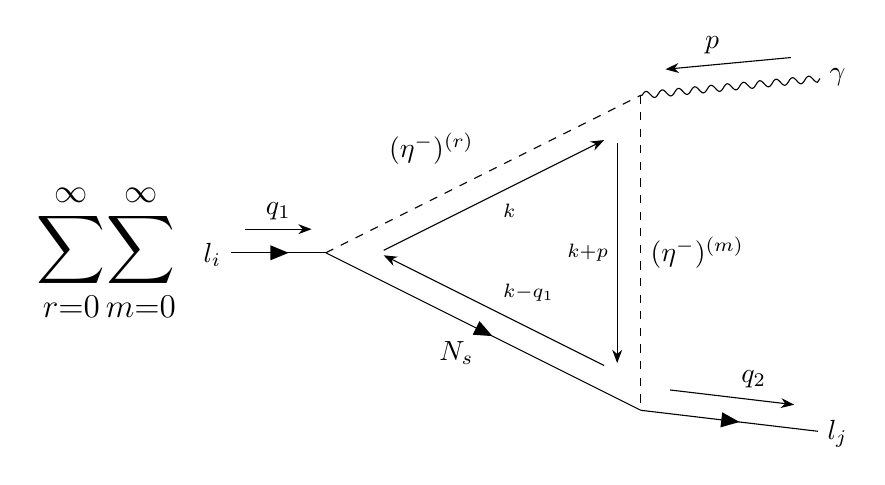
\begin{tikzpicture}
\begin{feynman}
\vertex (i) {\( \mathlarger{\mathlarger{\mathlarger{\mathlarger{\sum^{\infty}_{r=0}}}}}\mathlarger{\mathlarger{\mathlarger{\mathlarger{\sum^{\infty}_{m=0}}}}} \quad l_i \)};
\vertex[right=2.5cm of i] (a);
\vertex[right=4cm of a] (aux1);
\vertex[above=2cm of aux1] (b);
\vertex[below=2cm of aux1] (c);
\vertex[right=2.5cm of aux1] (aux2);
\vertex[above=2cm of aux2] (f1) {\(\gamma\)};
\vertex[below=2cm of aux2] (f2) {\(l_j\)};
\diagram*{
(i) -- [fermion, momentum=\(q_1\)] (a) -- [fermion, edge label'=\(N_s\), rmomentum=\(\mathsmaller{k-q_1}\)] (c) -- [fermion, momentum=\(q_2\)] (f2),
(a) -- [scalar, edge label=\((\eta^{-})^{(r)}\), momentum'=\(\mathsmaller{k}\)] (b) -- [photon, rmomentum=\(p\)] (f1),
(b) -- [scalar, edge label=\((\eta^{-})^{(m)}\), momentum'=\(\mathsmaller{k+p}\)] (c),
};
\end{feynman}
\end{tikzpicture}
\vspace{-3ex}
\caption{One-loop diagram to be calculated for \(l_i \rightarrow l_j \gamma\).}
\label{fig:egamma5D}
\end{figure}
From fig. \ref{fig:egamma5D}, we can infer the following three-point function,
\begin{equation}
\begin{aligned}
\Gamma^{\mu} = - P_L \sum_s \sum^{\infty}_{r=0} \sum^{\infty}_{m=0}
e^{\eff}_{rm} h^{\eff}_{is,r0} h^{\eff *}_{js,m0} \int \frac{\mu^{4 - D}\md^D k}{(2\pi)^D} 
\frac{(2k^{\mu} + p^{\mu})(\slashed{k} - \slashed{q_1})}{[k^2 - m^2_{\eta,r}][(k + p)^2 - m^2_{\eta,m}][(k-q_1)^2 - M^2_s]}.
\end{aligned}
\end{equation}
As each of the masses can be different this time, the integral we'll get at is more involved. The only
difference will reside in \(\Delta\), something that can be seen in eq. (\ref{eq:deltaemu}),
while numerator manipulations are unchanged. These differences start to make themselves evident when
integrating over Feynman parameters in eq. (\ref{eq:intemu}), which now reads
\begin{equation}
\begin{aligned}
\begin{gathered}
\frac{\mi}{16\pi^2} \sum_s \sum^{\infty}_{r=0} \sum^{\infty}_{m=0} e^{\eff}_{rm} h^{\eff}_{is,r0} h^{\eff *}_{js,m0}
\int^1_0 \md z \int^{1-z}_0 \md y \: \frac{z(y (m_i - m_j) + (z-1) m_i)}{(1-y-z)m^2_{\eta,r} + ym^2_{\eta,m} + zM^2_s} \\
\approx -\frac{\mi m_i}{16\pi^2} \sum_s \sum^{\infty}_{r=0} \sum^{\infty}_{m=0} e^{\eff}_{rm} h^{\eff}_{is,r0} h^{\eff *}_{js,m0}
\int^1_0 \md z \frac{z}{m_{\eta,m}^2 - m_{\eta,r}^2} \Bigg[1 - z \\
+ (M^2_s z - m_{\eta,m}^2 z + m_{\eta,m}^{2})\Bigg( \frac{ \ln{(M^2_s z - m_{\eta,r}^2 z + m_{\eta,r}^2 )}}
{m^2_{\eta,m} - m^2_{\eta,r}} \\
- \frac{\ln{(M^2_s z - m_{\eta,r}^2 z
+ m_{\eta,r}^2 + (1 - z) (m_{\eta,m}^2 - m_{\eta,r}^2))}}
{m^2_{\eta,m} - m^2_{\eta,r}}\Bigg)\Bigg].
\label{eq:LFV5D}
\end{gathered}
\end{aligned}
\end{equation}
The integral over \(z\) is not trivial, so numerical methods will be necessary here. There is a
worrying feature that we observe right away: the masses are exactly the same for equal indices
(and not approximately as was the case with \(m_{R,n}\) and \(m_{I,n}\)) so at first sight we spot
this expression diverging for such values. The easiest way to see that it is finite is to merely
do two different sums; one for \(m \neq r\), with the sum displayed on eq. (\ref{eq:LFV5D}),
and one with \(m = r\), using the expression in eq. (\ref{eq:intemu}), since we can stop ourselves
before integrating over \(y\), see that \(m_{\eta,m} = m_{\eta,r}\), have \(y\) vanish in the
denominator and proceed as we did in the rest of appendix \ref{app:lfv}.

It is likely that we will encounter a similar reduction of \(F_2(p^2)\) and \(F_3(p^2)\) as to what
we found in section \ref{sec:massmat5D}, given that these couplings will also be lowered due to
the wavefunctions they contain, and the interplay of parameters. However, the exact extent of such a
reduction, or even a possible enhancement, will require additional efforts.

\chapter{Conclusions}
% Repeat introduction, point out what can be done in the future.
In this Thesis, we have implemented an embedding of the scotogenic model in the Randall-Sundrum
scenario, placing the \(\eta\) doublet and the fermionic singlets \(N_s\) of the former in the
bulk. We chose a boundary condition for said fermions that leads to a particularly minimal albeit
more restrictive situation. Otherwise, the SM was left confined to the IR-brane. We have explored
the implications of the interaction between an IR-brane-confined SM Higgs with the fields conforming
\(\eta\), having shown that there exists a sizeable mass splitting between \(\eta^+\), \(\eta^0_R\)
and \(\eta^0_I\), which decreases as higher KK-modes are considered until reaching a certain value.

We have specified how we could build effective couplings, which are analogues to couplings in the
original scotogenic model, by absorbing the value of the five-dimensional wavefunctions into them,
as well as other relevant parameters of the theory. We have calculated two important processes in
the context of the scotogenic model, and promptly used them and said effective couplings to obtain
their counterparts in this embedding through the use of the effective four-dimensional theory coming
from a five-dimensional action after performing a KK-reduction. We have then observed several
differences with respect to the original scotogenic model which lead us to conclude that formally,
this embedding does not possess many differences, however the sum of multiple diagrams with similar
values of (non-effective) couplings to the original ScM actually leads to a possible decrease of both
neutrino masses and the branching ratio of \(\mu \rightarrow e \gamma\). While in the latter case,
such a decrease could be problematic, as it would worsen hopes for detection, the implications of
the former lead to a possible increase of \(\lambda_5\) or \(M_s\) in order to fit experimental data
with respect to the 4D case.

Future work along these lines ought to include further investigation into fitting these amplitudes
to experimental data, as well as studying the behaviour of the amplitude we calculated in
\ref{sec:lfv5D}, as part of an exhaustive phenomenological analysis of the implications of this
embedding. Such an analysis would explore the interplay of bounds from relic density observations
assuming \(N_1\) as dark matter, lepton flavor violation and lepton number violation bounds, as well
as data from active neutrino masses, which will allow to place constraints on Yukawa couplings,
\(M_1\), as well as the RS scenario's parameters.

\appendix
\chapter{Calculating the neutrino mass matrix in the scotogenic model}
\label{app:massmat}
Calculating the reduced amplitude through the use of the Feynman diagram in
figure \ref{fig:scmmass2} yields
\begin{equation}
\begin{aligned}
\mi \mathcal{M} = \overline{u}_{\nu_j}(p, r)\sum_{s}\int\frac{\mu^{4-D}\md^{D}k}{(2\pi)^{D}} 
\Bigg[\frac{\mi}{(p + k)^{2} - m^{2}_{R}} (\mi h_{js} P_L) \frac{\mi (\slashed{k} + M_{s})}{k^{2} - M^{2}_{s}} (\mi h_{is} P_L) \\
+ \frac{\mi}{(p + k)^{2} - m^{2}_{I}} (h_{js} P_L) \frac{\mi (\slashed{k} + M_{s})}{k^{2} - M^{2}_{s}}(h_{is} P_L)\Bigg]
u_{\nu_i}(p, r),
\end{aligned}
\end{equation}
where \(P_L = \frac{1}{2}(1 - \gamma_5)\) is the left-handed chirality projector,
\(D = 4 - \epsilon\) and \(\epsilon \rightarrow 0\) as we're using dimensional regularization. We
also included the energy scale \(\mu\) such that \(\mu^{4-D} \md^D k\) is dimension 4 in energy.
The radiative correction to the neutrino propagator is this amplitude after the previous
considerations and without the external line factors, these being the neutrino bispinors,
\begin{equation}
-\mi \Sigma(p^{2}) = -\sum_{s}h_{is}h_{js}\int \frac{\mu^{4-D}\md^D k}{(2\pi)^D}\left[
\frac{\mi}{(p + k)^{2} - m^2_R} \frac{\mi M_s}{k^2 - M^2_s}
- \frac{\mi}{(p + k)^{2} - m^2_I} \frac{\mi M_s}{k^2 - M^2_s}\right].
\end{equation}
We see that we really only have to solve one integral, up to the mass of the scalar in the loop.
This integral is
\begin{equation}
\int \frac{\mu^{4-D}\md^{D}k}{(2\pi)^{D}} \frac{M_{s}}{[(p + k)^{2} - m^{2}_{R}][k^{2} - M^{2}_{s}]},
\end{equation}
so now we make use of the Feynman parametrization,
\begin{equation}
\frac{1}{AB} = \int^1_0 \md x \: \frac{1}{(xA + (1-x)B)^2}; \quad A = (p + k)^2 - m^2_R, \quad B = k^2 - M^2_s,
\end{equation}
which yields
\begin{equation}
\int \frac{\mu^{4-D} \md^D k}{(2\pi)^D}\int^1_0 \md x \: \frac{M_s}{[((p + k)^2 - m^2_R)x + (k^2 - M^2_s)(1 - x)]^2}.
\end{equation}
Now, we need to manipulate the denominator a bit,
\begin{equation}
\begin{aligned}
\begin{gathered}
((p+k)^2 - m^2_R)x + (k^2 - M^2_s)(1-x) = p^2 x + k^2 x + 2(pk)x - m^2_R x + k^2 - k^2 x - M^2_s + M^2_s x \\
% Need to change p-k to p+k from here on out.
= (k + px)^2 - p^2 x(x-1) + M^2_s(x-1) - m^2_R x \equiv l^2 - \Delta,
\end{gathered}
\end{aligned}
\end{equation}
where we defined \(l = k + px\) and \(\Delta = m^2_R x - (p^2 x - M^2_s)(1 - x)\). The resulting
integral is
\begin{equation}
\begin{aligned}
\begin{gathered}
M_{s}\mu^{4-D} \int^1_0 \md x \: \int \frac{\md^D k}{(2\pi)^D} \frac{1}{(l^2 - \Delta)^2}.
\end{gathered}
\end{aligned}
\end{equation}
Knowing that
\begin{equation}
\int \md^{D}k \frac{1}{(l^2 - \Delta)^N} = \mi (-1)^N \pi^{\frac{D}{2}} \frac{\Gamma(N - \frac{D}{2})}{\Gamma(N)}\Delta^{\frac{D}{2}-N},
\label{eq:intrenor}
\end{equation}
we evaluate the integral with respect to \(l\), use standard manipulations, and arrive at
\begin{equation}
\begin{aligned}
\begin{gathered}
\frac{\mi M_{s}}{(4\pi)^{2}} \left(\frac{2}{\epsilon} - \gamma_{E} + \ln 4\pi - \int^{1}_{0} \md x \ln \frac{\Delta}{\mu^2} \right).
\end{gathered}
\end{aligned}
\end{equation}

We shall set \(p^2 = 0\) now,
\begin{equation}
\begin{aligned}
\begin{gathered}
\frac{\mi M_s}{(4\pi)^2} \int^1_0 \md x \ln \frac{\Delta}{\mu^2} \approx 
\frac{\mi M_s}{(4\pi)^2} \int^1_0 \md x \ln \left[\frac{m^{2}_{R}x + M^2_s(1-x)}{\mu^2}\right] \\
= \frac{\mi M_s}{(4\pi)^{2}} \left(\frac{M^{2}_{s}\ln \frac{M^2_s}{\mu^2} - m^2_R\ln \frac{m^2_R}{\mu^2} + m^2_R - M^2_s}{M^2_s - m^2_R}\right) \\
= \frac{\mi M_s}{(4\pi)^{2}} \frac{m^2_R}{m^2_R - M^2_s}\ln \frac{m^2_R}{M^2_s}.
\label{eq:asss}
\end{gathered}
\end{aligned}
\end{equation}
Now, all we need to obtain the resulting correction to the mass is to do this again, but with
\(\eta^0_I\) rather than \(\eta^0_R\) as we have just done, and to sum their contributions.
The only difference is the scalar particle's mass, so the result is
\begin{equation}
\begin{aligned}
\begin{gathered}
(m_{\nu})_{ij} = \sum_{s}\frac{h_{is}h_{js} M_s}{16\pi^2}\left( \frac{m^2_R}{m^2_R - M^2_s}\ln \frac{m^2_R}{M^2_s} -
\frac{m^2_I}{m^2_I - M^2_s}\ln \frac{m^2_I}{M^2_s} \right).
\label{eq:massmatap}
\end{gathered}
\end{aligned}
\end{equation}
Let's stop here for a second and appreciate that eq. (\ref{eq:massmatap}) is finite, which is
due to the fact that the two sorts of diagrams here, each with a different scalar and opposite sign,
have their divergent parts cancel each other out without resorting to renormalization.\footnote{This
is not surprising, as a power counting on the diagram in fig. \ref{fig:scmmass1} reveals that there
is no divergence, and EWSB does not introduce divergences.}

\chapter{Calculating \(\mu \rightarrow e \gamma\) in the scotogenic model}
\label{app:lfv}
The reduced amplitude for this process is
\begin{equation}
\begin{aligned}
\mi \mathcal{M} = \varepsilon^*_{\mu}(p, \lambda) \overline{u}_{l_j} (q_2, r_2) \Bigg[\sum_s \int \frac{\mu^{4 - D}\md^D k}{(2\pi)^D} 
\frac{\mi}{k^2 - m^2_{\eta}}(\mi e (2k + p)^{\mu})\frac{\mi}{(k + p)^2 - m^2_{\eta}} \\
\times (\mi h^*_{js} P_R) \frac{\mi(\slashed{k} - \slashed{q_1} + M_s)}{(k-q_1)^2 - M^2_s} (\mi h_{is} P_L) \Bigg] u_{l_i} (q_1, r_1),
\end{aligned}
\end{equation}
so the three-point function is
\begin{equation}
\begin{aligned}
\Gamma^{\mu} = - e P_R \sum_s h_{is} h^*_{js} \int \frac{\mu^{4 - D}\md^D k}{(2\pi)^D} 
\frac{(2k^{\mu} + p^{\mu})(\slashed{k} - \slashed{q_1})}{[k^2 - m^2_{\eta}][(k + p)^2 - m^2_{\eta}][(k-q_1)^2 - M^2_s]}.
\end{aligned}
\end{equation}
Following \cite{peskshro} we press on with the use of the Feynman parametrization;
\begin{equation}
\begin{aligned}
\frac{1}{ABC} &= \int^1_0 \md x \int^1_0 \md y \int^1_0 \md z \: \delta(x + y + z - 1) \frac{2}{(xA + yB + zC)^3} \: ; \\[7pt]
A &= k^2 - m^2_{\eta}, \: B = (k + p)^2 - m^2_{\eta}, \: C = (k-q_1)^2 - M^2_s,
\label{eq:feynparam3}
\end{aligned}
\end{equation}
so we take the resulting denominator and manipulate it to make it a bit more palatable,
\begin{equation}
\begin{aligned}
\begin{gathered}
x[k^2 - m^2_{\eta}] + y[(k + p)^2 - m^2_{\eta}] + z[(k-q_1)^2 - M^2_s] \\
= (k + yp - zq_1)^2 - y^2 p^2 - z^2 q^2_1 + 2yz(pq_1) + yp^2 + zq^2_1 + (z-1) m^2_{\eta} - zM^2_s \equiv l^2 - \Delta,
\label{eq:deltaemu}
\end{gathered}
\end{aligned}
\end{equation}
where we used that \(x + y + z = 1\) as per the Dirac delta in eq. (\ref{eq:feynparam3}). The integral
now takes the following form after changing variables,
\begin{equation}
\begin{aligned}
\begin{gathered}
- 2 e P_R \sum_s h_{is} h^*_{js} \int^1_0 \md x \: \md y \: \md z \: \delta(x + y + z - 1) \\
\times \int \frac{\mu^{4 - D}\md^D l}{(2\pi)^D}
\frac{(2l^{\mu} - 2yp^{\mu} + 2zq^{\mu}_1 + p^{\mu}) (\slashed{l} - y\slashed{p} + (z - 1)\slashed{q_1})}{(l^2 - \Delta)^3}.
\end{gathered}
\end{aligned}
\end{equation}
We now need to massage this numerator a bit in order to carry out the calculation,
\begin{equation}
\begin{aligned}
\begin{gathered}
(2l^{\mu} - 2yp^{\mu} + 2zq^{\mu}_1 + p^{\mu}) (\slashed{l} - y\slashed{p} + (z - 1)\slashed{q_1}) \\
= \gamma_{\nu} (2l^{\mu}\slashed{l} - 2y l^{\mu} \slashed{p} + 2(z-1)l^{\mu}\slashed{q_1}
+ (1 - 2y)(p^{\mu}\slashed{l} - yp^{\mu}\slashed{p} + (z-1)p^{\mu}\slashed{q_1}) \\
+ 2zq^{\mu}_1 \slashed{l} - 2yz q^{\mu}_1 \slashed{p} + 2z(z-1) q^{\mu}_1 \slashed{q_1}).
\label{eq:numerator1}
\end{gathered}
\end{aligned}
\end{equation}
Terms in eq. (\ref{eq:numerator1}) which are proportional to \(l^{\mu}\) vanish when integrating,
as is usual in these sorts of integrals. Making use of Lorentz invariance, as such,
\begin{equation}
\begin{aligned}
\int \frac{\md^D l}{(2\pi)^D} l^{\mu} l^{\nu} = \int \frac{\md^D l}{(2\pi)^D} \frac{l^2 \eta^{\mu \nu}}{D},
\end{aligned}
\end{equation}
we now get
\begin{equation}
\begin{aligned}
\begin{gathered}
\frac{1}{2}l^2\gamma^{\mu} + (1 - 2y)(- yp^{\mu}\slashed{p} + (z-1)p^{\mu}\slashed{q_1})
- 2yz q^{\mu}_1 \slashed{p} + 2z(z-1) q^{\mu}_1 \slashed{q_1},
\end{gathered}
\end{aligned}
\end{equation}
and if we apply the equations of motion for the bispinors, we can get rid of these slashed momenta,
replacing them for their corresponding masses.
\begin{equation}
\begin{aligned}
\begin{gathered}
\frac{1}{2}l^2\gamma^{\mu} + (1 - 2y)(- y(m_j - m_i) + (z-1)m_i) p^{\mu}
- 2yz q^{\mu}_1 (m_j - m_i) + 2z(z-1) q^{\mu}_1 m_i.
\end{gathered}
\end{aligned}
\end{equation}
We shall also plug in \(q_1 = \frac{1}{2}q_1 + \frac{1}{2}q_1 = \frac{1}{2}q_1 + \frac{1}{2}(q_2 - p)
= \frac{1}{2}(q_1 + q_2 - p)\), as we wish to make this into a linear combination of \(\gamma^{\mu}\),
\(p^{\mu}\) and \((q_1 + q_2)^{\mu}\) in order to utilize relations akin to the Gordon identity, so
\begin{equation}
\begin{aligned}
\begin{gathered}
\frac{1}{2}l^2\gamma^{\mu} + (1 - 2y)(- y(m_j - m_i) + (z-1)m_i) p^{\mu}
+ 2z(- y (m_j - m_i) + (z-1) m_i)q^{\mu}_1 \\
= \frac{1}{2}l^2\gamma^{\mu} + (1 - 2y - z)(- y(m_j - m_i) + (z-1)m_i) p^{\mu}
+ z(- y (m_j - m_i) + (z-1) m_i)(q_1 + q_2)^{\mu}.
\label{eq:numerator2}
\end{gathered}
\end{aligned}
\end{equation}
Up until now we have ignored \(P_R\); when we multiply eq. (\ref{eq:numerator2}) with \(P_R\), we
will have a vector and an axial-vector contribution. We shall now focus on the vector contribution,
and within it, calculate the integral which is a factor to \((q_1 + q_2)^{\mu}\), which is
\(- \frac{\mi e}{2m_i}F_2(p^2)\). Such a form factor should be evaluated at \(p^2 = 0\), as can be
seen in eq. (\ref{eq:aral}). Setting this greatly simplifies the final expression for the integral
over \(y\). The aforementioned integral is
\begin{equation}
\begin{aligned}
\begin{gathered}
- 2 e \sum_s h_{is} h^*_{js} \int^1_0 \md z \int^{1-z}_0 \md y \int \frac{\mu^{4 - D}\md^D l}{(2\pi)^D}
\frac{z(y (m_i - m_j) + (z-1) m_i)}{(l^2 - \Delta)^3}.
\end{gathered}
\end{aligned}
\end{equation}
Using eq. (\ref{eq:intrenor}), we see that
\begin{equation}
\begin{aligned}
\mu^{4-D} \int \frac{\md^D l}{(2\pi)^D} \frac{1}{(l^2 - \Delta)^3} = \frac{\mu^{4 - D} (-1)^3 \pi^{D/2}}{(2\pi)^D}
\frac{\Gamma\left(3 - \frac{D}{2}\right)}{\Gamma(3)}\Delta^{\frac{D}{2} - 3}.
\end{aligned}
\end{equation}
If we make \(D \rightarrow 4\), through the usual parametrization, \(D = 4 - \epsilon\), \(\epsilon \rightarrow 0\),
we obtain
\begin{equation}
\begin{aligned}
- \mi \mu^{\epsilon} \pi^{\frac{\epsilon}{2} - 2} 2^{\epsilon - 5} \Gamma\left(1 - \frac{\epsilon}{2}\right)\Delta^{-1-\frac{\epsilon}{2}}
= - \frac{\mi}{32\pi^2} \frac{1}{\Delta}.
\label{eq:firkind}
\end{aligned}
\end{equation}
There is no divergence here either, since the only source of this was the evaluation of the gamma function at one
of its poles, which does not take place in this case. So, the whole integral is now

\begin{equation}
\begin{aligned}
\begin{gathered}
- 2 e \sum_s h_{is} h^*_{js} \int^1_0 \md z \int^{1-z}_0 \md y \: z(y (m_i - m_j) + (z-1) m_i)
\left(- \frac{\mi}{32\pi^2} \frac{1}{\Delta}\right) \\
\approx \frac{\mi e}{16\pi^2} \sum_s h_{is} h^*_{js} \int^1_0 \md z \int^{1-z}_0 \md y \: \frac{z(y (m_i - m_j) + (z-1) m_i)}{m^2_{\eta} + z(M^2_s - m^2_{\eta})} \\
\approx [m_i \gg m_j] \approx -\frac{\mi e m_i}{32\pi^2 m^2_{\eta}} \sum_s h_{is} h^*_{js} \int^1_0 \md z \: \frac{z(1-z)^2}{x_s z - z + 1} \\
= \frac{\mi e m_i}{16\pi^2 m^2_{\eta}} \sum_s h_{is} h^*_{js} \left(\frac{1 - 6x_s + 3x_s^2 + 2x_s^3 - 6x_s^2 \ln x_s}{6(1-x_s)^4}\right),
\label{eq:intemu}
\end{gathered}
\end{aligned}
\end{equation}
where \(x_s \equiv M^2_s/m^2_{\eta}\).

\chapter*{Bibliography}
\addcontentsline{toc}{chapter}{Bibliography}

\begin{multicols}{2}
\printbibliography[heading=none]
\end{multicols}

\end{document}
